\documentclass[12pt]{report}
\usepackage[margin=1in]{geometry} % change margins
\usepackage{graphicx} % inserting images
\usepackage{caption} % captions
\usepackage{amsmath} % for better math
\usepackage{verbatim} %used for comment blocks
\usepackage{mathtools}
\usepackage[english]{babel}
\usepackage[colorinlistoftodos]{todonotes}
\usepackage{placeins}
\usepackage[square, sort, numbers]{natbib}
\usepackage{url}
\usepackage{setspace}
\usepackage{breqn}
\usepackage{subcaption}
\usepackage{textcomp}
\usepackage{float}
\usepackage{leftidx}
\usepackage{bm}
\usepackage[titletoc,toc, title]{appendix}
\usepackage[utf8]{inputenc}
\usepackage{diagbox}
\usepackage{hyperref}
\usepackage{tcolorbox}

\usepackage{amsmath,amssymb,braket,cancel,nicefrac,physics,tensor,slashed}
\usepackage{color,empheq,enumitem,forloop,graphicx,microtype,subcaption,verbatim,wrapfig,pdfpages,titlesec}
\usepackage{array,booktabs,multicol,multirow,tabularx} 

\usepackage{fancyhdr}
\addto\captionsenglish{\renewcommand{\chaptername}{Lab}}
\setcounter{chapter}{-1}

\def\cesar#1{{\color{blue}[#1]}}
\def\anhkhoi#1{{\color{olive}[#1]}}
\def\nik#1{{\color{red} [#1]}}

\tcbset{colback=blue!5!white,colframe=blue!75!black,center,halign=justify,width=0.9\textwidth,fonttitle=\bfseries}

\linespread{1.15}
\title{PHYS 102: TA Lab Manual}
\author{Nikolas Provatas, Anh-Khoi Trinh}

\begin{document}
\maketitle

\tableofcontents

\phantomsection
\addcontentsline{toc}{part}{Introduction}
\part*{Introduction} \label{Sec:Intro}

\phantomsection
\addcontentsline{toc}{chapter}{Lab Format}
\chapter*{Lab Format}

\phantomsection
\addcontentsline{toc}{section}{Introduction, Learning Objectives and Lab Structure}
\section*{Introduction, Learning Objectives and Lab Structure}
Welcome to PHYS 102! The focus of these lab session will be to teach you how to think critically about  data collected from experiments, a skill that can be applied in many other STEM fields and in your own personal lives. You will learn how to acquire and analyse data quantitatively in experiments pertaining to electromagnetism experiments. \\

\noindent \large \textbf{Learning objectives} \normalsize

Whether it is in your professional or personal lives, the ability to analyse and think critically about information, particularly information in the form of data, is a valuable one. In an age where one can feel overwhelmed by the prevalence of information from documentaries, non-fiction books, online websites and politicians, one must find a way to sift through this sea of information to determine objective truths. As scientists, we recommend the \textit{scientific method}.

While the labs will be related to electromagnetism topics that you will learn about in class, the main focus of these labs will be for you to be acquainted with the scientific method. This methodology will be used to answer a question posed to you through data collected and observations you make. The first step is to conjecture a \textit{falsifiable} hypothesis to answer this question. One then performs an experiment to verify said hypothesis. After that, one can make a conclusion based on the data. In these labs, you will be asked to apply the scientific method \underline{quantitatively} to electromagnetism experiments. \\

\noindent \large \textbf{Lab structure} \normalsize

In these labs, you will have two 2-hour sessions to complete your labs: one session per week over the span of two weeks. You will have different tasks to accomplish per session. The goal of this two-session setup is to allow students to make mistakes during the first session, think critically about these, and improve your experimental data and or interpretation of these in the second session. Contrary to other lab courses that you may have taken, the emphasis here is to evaluate a student's critical thinking \textit{process}. This is best achieved when acquiring crude or bad data at first, and leaving room for follow up and subsequent improvement. The critical thinking process of improving one's data is the main focus of these labs.

To evaluate a student's critical thinking process, we will resort to the following grading rubric:
\begin{itemize}
\item $15 \%$ for attendance (to both sessions of a given lab)
\item $15 \%$ for a pre-lab analysis
\item $10 \%$ for participation in group discussions
\item $60 \%$ for the content of your log book
\end{itemize}

Given the focus on critical thinking, the instructions for each lab will be minimal. Students must learn how to acquire meaningful data on their own. Their thinking process must therefore be reflected in their log book with enough clarity, organization and precision to allow us evaluate their ability to think critically. TAs will be more involved that in typical labs in order to guide students throughout the labs.

At the start of the first session, each student will be asked to submit their pre-lab answers to specific questions posed. Students will then be asked to divide into pairs and perform  measurements as a team to collect data related to the posed question(s). All methods, experimental data collected, and interpretations will be written in log book. By the end of the first session, students are asked to hand in \underline{a single} log book \underline{per team}. While you cannot bring the log book home, you are allowed (and encouraged) to take pictures of the log book to think about your results between the two sessions and plan ahead what you intend to do in the second session to improve your experiments. Although you will work with one teammate, and submit one joint journal, as is common in scientific research, we highly encourage discussions with other teams and students outside of the lab session. Such discussions will start in the lab, where TAs will facilitate group discussions between groups to help students troubleshoot their experiments and understand sources of error. You will receive your log book again at the start of the second session to document your improved experiment, new data collected and any revised interpretations. By the end of the second session, students will again submit their log book for evaluation. For most labs, there will be an individual work station and a collective work station. The former offers the base materials and supplies for each group to successfully finish the lab, while the collective work station offers additional material that can be used to improve your data.

\phantomsection
\addcontentsline{toc}{section}{Lab Log Look}
\section*{Lab Log Books}
The log book will be your primary source of evaluation. You will be asked to submit a log book entry by the end of each session. We will distribute at the start of each session the following structured log book:
 
\noindent \textbf{i) Introduction (5\%)}\\
\noindent Clearly state your goal. This can be a brief re-statement of the question, or of your method to improve your data. Clearly state your hypotheses. Write down what you intend to verify experimentally, and why this method is an appropriate verification of your hypothesis. This part may differ for the second session since you may be more acquainted with the theory and experiment. \\

\noindent \textbf{ii) General Notes: Methodology and Rough data (35\%)}\\
In this section, we expect you to write all your observations so that we can see your thought process as you are performing the lab. 

As opposed to other lab reports that you may have submitted, we do not expect a clean point-by-point list of manipulations. In fact, you may start following a set of protocol and realize you made some mistakes and therefore should change your original protocol. We recommend writing short sentences and/or intelligible and readable notes of what your are doing. If you do encounter unexpected problems, please write down what they were, and how you resolved them.

We encourage you to write your measurements and rough calculations as you do your measurements. If you choose to compile your data in Excel, you should simply write a few sample calculations. These sample calculations do not need to follow the significant figure rules to be outlined later. More importantly, \textbf{you should write down \underline{all} your observations}. This part can be messy, but as long as the information that you want to convey is clear. We recommend boxing, colouring, underlining and/or labelling important measurements, calculations or observations. \\

\noindent \textbf{iii) Results (30\%)}\\
\noindent In this section, you will present your data \underline{in its most presentable form}. This differs from the previous section by the way that you present your data: significant figures, graph rules, etc. have to be followed. You will also state your observation and analysis in this part. We expect you to be able to present your data adequately according to instructions from the \textbf{Data Analysis} section. For electronic files such as Excel documents, a TA will have a USB drive onto which you are to upload your documents.\\

\noindent \textbf{iv) Conclusions and future work (30\%)}\\
\noindent In this section, you will state your conclusion, and offer possible follow-ups to this lab. This can include other physical properties to study, or to offer a better methodology to study this phenomenon. You must motivate your proposed follow-up project by clearly stating what you expect to observe (a hypothesis) and support your claim based on your current experiment. The proposed future projects must be realistically performed by your peers, and must not assume an unrealistic sum of budgetary support or higher level of experimental expertise such that you or your peers are not acquainted to. For your lab report submitted at the end of the first session, be mindful that you must execute your proposed improvements during the second session.

\phantomsection
\addcontentsline{toc}{chapter}{Data Analysis}
\chapter*{Data Analysis}

\phantomsection
\addcontentsline{toc}{section}{General Guidelines}
\section*{General Guidelines}
Here is a list of general guidelines for your log book:
\begin{itemize}
\item Measurements must always include \textbf{units}.
\item Measurements must include an uncertainty (\textbf{standard deviation}).
\item Tables (and any other data representation method) must also include appropriate labels, units and standard deviation.
\item When comparing to a known quantity (theoretical value), the former does not have a standard deviation attributed to it, unless that information is found from an experiment, in which case there should be an associated standard deviation.
\item If you quote results from elsewhere, you must include the source: \anhkhoi{how to quote sources}
\item Recall that vector-data has both a \textbf{magnitude} and a \textbf{direction}.
\item Write down \underline{all} your observations and some commentary about them.
\end{itemize}

\noindent Figures must
\begin{itemize}
\item Include a title.
\item Include labels on your axes.
\item Include units on your axes.
\item Include a few tick markers for the audience to know the scale.
\item Use an appropriate scale.
\item Include a legend for the different curves shown on a single plot.
\item Fit equation (and $R^2$ value) if a fit was used.
\item Not have joint data points (unless necessary).
\end{itemize}

\phantomsection
\addcontentsline{toc}{section}{Data Presentation}
\section*{Data Presentation}
One of the most important aspects of doing research is to be able to communicate efficiently your findings. In physics, this is done mostly by means of one of the following:
\begin{itemize}
\item A quoted result
\item A table of results
\item A figure
\end{itemize}

As emphasized previously, all quoted results must include an uncertainty i.e. a standard deviation and units. For example, if I measured the gravitational acceleration, I can quote it as
\begin{equation}
g = 9.8 \pm 0.2 \ m/s^2.
\end{equation}
Usually, if you have a single result, you must explain what it is: was it from a single measurement? Was it an average or did you obtain it from some other method? Whatever the method that you used, there is a specific way to obtain the correct uncertainties. This will be explained in the next sections.

On rare occasions, there are certain quantities that do not need a standard deviation. This could include percentages of error or absolute error differences.

If you choose to present multiple results, you may opt for a table. In this case, you still must include standard deviations and units.
\begin{table}[h]
\centering
\begin{tabular}{||c|c||}
\hline
Voltage ($\pm 0.2$ V) & Current ($\pm 0.1$ A) \\ \hline
3 & 15 \\
5 & 25 \\
7 & 35 \\ \hline
\end{tabular}
\caption{Example of a table where all measurements have the same standard deviation. If they didn't, you must still include them individually.}
\label{Table:Presentation-Example}
\end{table}

Tables are useful to show the explicit values of your results. However sometimes the exact values aren't as important as the general trend. In this case, you would opt to present your data in chart form.

There are many types of possible charts. The most useful one for us will be the scatter plot. An example of a scatter plot is shown in Fig.~\ref{Fig:Example-Scatter}.
\begin{figure}[h]
\centering
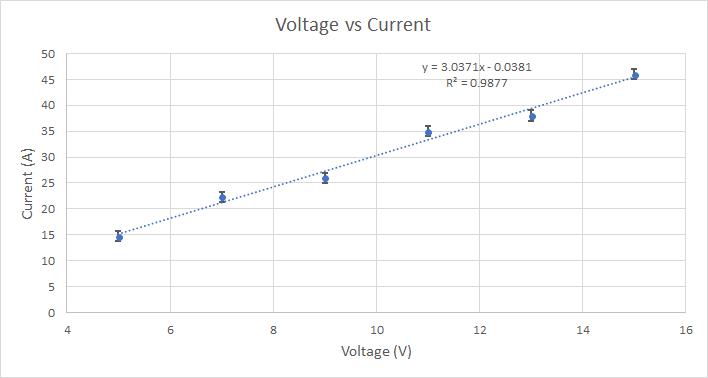
\includegraphics[width=0.9\textwidth]{intro-example-scatter}
\caption{Example of a scatter plot. Each measurement is displayed as a point. One can add error bars in both the x and y axes (although only the y direction is displayed here). One can also fit an equation to the data set.}
\label{Fig:Example-Scatter}
\end{figure}

A scatter plot allows you to see the general trend of your data. If you expect a specific behaviour, you can fit a trendline to your data to match a specific equation. By further plotting error bars, you can compare how far away your data points are from the expected trendline. This gives you some insight into whether your data matches your expected trend. From the trendline, you can also see the actual coefficient of the fit. As shown in Fig.~\ref{Fig:Example-Scatter}, you can also display a $R^2$ value, which is called the coefficient of determination. This tells you how good your fit was to your data. A good $R^2$ value is $1$. For the example of Fig.~\ref{Fig:Example-Scatter}, the $R^2$ value is good and most of the measurements fall within a standard deviation of the fit, therefore this says that the current is proportional to the voltage by a proportionality factor of $3.0371$. 

In summary, to present your data, you will need to know certain things: how to perform an average and other basic statistics, how to evaluate the uncertainty in your measurements and by extension, your final result, how many digits to display in your final answer, and most importantly, how to analyse your data. This will be the subject of the following sections.

\phantomsection
\addcontentsline{toc}{section}{Basic Statistics}
\section*{Basic Statistics}

\noindent \large \textbf{Mean} \normalsize

Let $y(x)$ be a function of $x_i$ datapoints. The value of $y$ for $x_i$ can be denoted by $y(x_i)$ or $y_i$. The mean, or average, denoted by $\bar{y}$ of a dataset with $N$ datapoints is given by
\begin{equation}
\bar{y} = \frac{1}{N} \displaystyle \sum_{i}^N y(x_i) = \frac{1}{N} \left( y(x_1) + y(x_2) +... + y(x_N) \right).
\end{equation}

\noindent \large \textbf{Standard deviation} \normalsize

The standard deviation of a function $y(x)$ is denoted by $\sigma_y$. One says that a measurement $y(x_i)$ has an \textit{uncertainty} of
\begin{equation}
y_i \pm \sigma_{y_i}.
\end{equation}
The standard deviation tells you up to what value is your data precise: your data point can vary between $y_i + \sigma_{y_i}$ and $y_i - \sigma_{y_i}$. This means that your measurement $y_i$ can vary by $2 \sigma_{y_i}$. A good set of measurement would have a very small standard deviation: this gives you the bounds under which your measurement is considered precise. You will see in section ``\textbf{Error Analysis}" how to quantify this quantity. \\

\noindent \large \textbf{Significant Numbers} \normalsize

To present results, one must present an appropriate number of significant numbers. In this course, we will not be concerned with the \textit{number of significant digits}, but more with the precision attributed to a measurement. When quoting a measurement, the last digit should be fixed by the uncertainty of the measurement: it must match the order of magnitude of the standard deviation. In other words, the standard deviation fixes up to what precision (roughly decimal place) you can quote your results. Table~\ref{Tab:SigFigs} lists some common mistakes and how to present those results appropriately. In the context of this course, we will simplify our conventions by \underline{keeping only one significant number for the standard deviation}. Recall that leading zeros do not count as a significant number and trailing zeros (after the precision of the standard deviation) should be discarded.

\begin{table}[h]
\centering
\begin{tabular}{||c|c||}
\hline
Incorrect & Correct \\ \hline
$324.9453 \pm 0.02$m & $324.95 \pm 0.02$m \\
$20 \pm 0.1$\$ & $20.0 \pm 0.1$\$ \\
$3 \times 10^4 \pm 2$N & $3000 \pm 2$N \\
$31.02 \pm 0.10$\$ & $31.0 \pm 0.1$\$ \\
$0.003564 \pm 0.00012$m/s & $0.0036 \pm 0.0001$m/s \\ \hline
\end{tabular}
\caption{Significant numbers. Common mistakes and the correct way to present such results.}
\label{Tab:SigFigs}
\end{table}

\noindent \large \textbf{Precision versus Accuracy} \normalsize

\textbf{Precision} refers to how closely related two measurements are from each other. This means that one expects a \underline{small standard deviation} for highly precise measurements.

\textbf{Accuracy} measurements refers to the closeness of a measurement from a \textit{known} value. This means that one must calculate the \underline{difference} of the measurement to the known value \underline{in terms of standard deviations}. For example, if $y=0.4 \pm 0.1$m, and the known value is $y_t=0.7$m, then the measurement differs by $3\sigma_y$.

Often, one may encounter a highly precise set of measurements, but also very inaccurate. This is a signal that there may have been a \textbf{systematic error} in your results. This is a type of error that propagates throughout your experiment and offsets your results by a constant factor. For example, recall the equation of the period of oscillation of a pendulum is
\begin{equation}
T = 2 \pi \sqrt{\frac{L}{g}}.
\end{equation}
If one incorrectly measured the length $L$ of the string, then the results would be offset by a constant factor of $\sqrt{L_{good}- L_{bad}}$. \\

\phantomsection
\addcontentsline{toc}{section}{Error Analysis}
\section*{Error Analysis} \label{Sec:ErrorAnalysis}

\noindent \large \textbf{Standard deviation of a measurement} \normalsize

The \textit{rule of thumb} for finding the standard deviation of measurements is as follows: each measurement can vary by \textit{half} of the smallest available precision from your measuring instrument, and you must add the uncertainties of the measurement. Consider the example of measuring a distance with a 30cm ruler. The smallest increment is a mm. When you measure a distance between \underline{two points}, you take \underline{two} measurements: one at each point. Thus the uncertainty on the measurement is $2 \times 0.5$mm, so $1$mm. This is exactly the smallest available increment of your measuring device. Therefore, unless otherwise specified, the \textit{standard deviation of a measurement is the smallest available measurable value allowed by your instrument}. 

Another example is measuring the time difference between two events. Again, there will be two measurements: the initial and end time. Stopwatches often allow one to view up to ms precision. However, the average visual time reaction is roughly $0.3$s, and therefore each initial and final time measurement varies by $0.15$s and so the uncertainty for the whole measurement is $0.3$s. \\

\noindent \textbf{Standard deviation for fluctuating data}

For fluctuating datasets where \textit{each measurement is independent of the previous}, to reliably represent your data, you should take some form of average over some number of measurements. Measurements that are random are said to follow a \textit{Poisson distribution}. To study these types of measurements, one typically chooses a subset of $N$ data points, and calculate its mean. Given the mean, one must approximate the error as
\begin{equation}
d_i = y_i - \bar{y}.
\end{equation}
The standard deviation on the average of your measurements will therefore be given as
\begin{equation}
\sigma_{\bar{y}} = \sqrt{ \frac{1}{N} \displaystyle \sum_{i=1}^{N} d_i^2}.
\label{Eq:STDev.P}
\end{equation}
This can be obtained in Excel by using the function \verb|=STDEV.P(x)|. \\

\noindent \large \textbf{Error propagation} \normalsize

The standard deviation value above is attributed to \underline{a single measurement}. However, often one would be interested in deriving a quantity that depends on \textit{multiple} measurements. To describe the standard deviation on the end result, one must use \textit{error propagation techniques}.

For these labs, you will only need to know the following two error propagation formulas. Consider first the following function
\begin{equation}
f(x,y) = x \times y.
\label{Eq:f=xy}
\end{equation}
The standard deviation $\sigma_f$ on $f$ will be
\begin{equation}
\sigma_f = \sqrt{ (x \sigma_y)^2 + (y \sigma_x)^2}.
\label{Eq:product error}
\end{equation}
This will be useful for example to calculate the error on the area given two length measurements, or in Lab 2, you can calculate the error on the time constant in a similar way.

Consider also the function
\begin{equation}
f(x) = \frac{1}{x}.
\label{Eq:f=1/x}
\end{equation}
The standard deviation for this case is
\begin{equation}
\sigma_f = \frac{\sigma_x}{x^2}.
\label{Eq:1/x error}
\end{equation}


\noindent \large \textbf{Measurement analysis} \normalsize

To understand the significance of a measurement, one can compare it in different ways. When a theoretical value is known, one can compare a set of measurements by calculating the \textit{absolute error}, the \textit{percentage error} or the \textit{standard deviation error}. One can also analyse a dataset by studying fits in a similar manner. \\

\noindent \textbf{Absolute error}

The absolute error indicates the difference between the known value, and either a measurement, the mean value of a set of measurements, or a fit parameter. One can also compare a set of measurement to the fit of the dataset in this matter. Let $y_t$ be the theoretical value and $y$ be one of the variables mentioned before, then the absolute value is
\begin{equation}
\text{Absolute error} = \left\rvert y_t - y \right\rvert
\end{equation}

\noindent \textbf{Percentage error}

The percentage error is simply the ratio of absolute error relative to the known value. This gives an indication, in percentage, of how far away with respect to the known value is the measurement. It is given as
\begin{equation}
\text{Percentage error} = \left\rvert \frac{y_t - y}{y_t} \right\rvert \times 100
\end{equation}

\noindent \textbf{Standard deviation error}

The standard deviation error indicates how many standard deviations away is a measurement when compared to the known value. It is given as
\begin{equation}
\text{Standard deviation error} = \left\rvert \frac{y_t - y}{\sigma_y} \right\rvert
\end{equation}

You will have to recognize which one of the above is useful and representative of the information that you wish to convey for the data analysis that you have to perform. Note that we've taken the absolute values of the above, but by not doing so, we could convey information about the ``direction" of the error i.e. whether the measurements are higher or lower than the known theoretical value.\\

\noindent \large \textbf{Fit analysis} \normalsize

As mentioned before, a good way to know whether your fit is correct is to compute the coefficient of determination $R^2$. To compare your fit to your data, you should see whether your data points all (or mostly) fall within one standard deviation of the fitted equation, that is if the standard deviation error should be less than 1 $\sigma$ for all data points when compared to $y_{fit}$.


\phantomsection
\addcontentsline{toc}{part}{Lab Manuals}
\part*{Lab Manuals} \label{Part:Labs}

\chapter{Data Analysis Practice}
\section{Learning objectives}
\begin{itemize}
\item Learn how to use Excel.
\item Compute certain basic mathematical statistics.
\item Introduction to data analysis.
\end{itemize}

\section{Introduction}
This lab will be an interactive demo lab where teaching Assistants will help you  learn how to use Excel and to apply it to the concepts presented in the \textbf{Data analysis} chapter. We recommend that you read the \textbf{Data Analysis} and familiarize yourself to Excel before attending this session. This lab will be called "Lab 0" and will be scheduled in the Lab information document on MyCourses. 

\section{Session a}
In this session, you will familiarize yourself with Excel. You will be guided through this exercise by the TAs.

\begin{itemize}
\item Open the Excel document found at \anhkhoi{location}.
\item Explore the user interface. Note that data is best presented in columns.
\item Learn how to resize, split and merge cells.
\item In a adjacent column, calculate the resistance $R$. 
\item Calculate the sum of resistances $R$ by using  \verb|=SUM(x)|.
\item Calculate the average resistance $\bar{R}$ in two ways: by using the integrated function  \verb|=AVERAGE(x)| and by dividing the sum that you calculated previously by the total number of cells.
\item For each value of resistance $R_i$, calculate the difference
\begin{equation}
R_i - \bar{R},
\end{equation}
in a separate column by ``dragging" the first cell downwards.

\item Calculated the square of the difference calculated above in another column.
\item In two other columns, calculate the standard deviation by using eq.~\eqref{Eq:STDev.P} with the values that you calculated previously, and by using the function \verb|=STDEV.P(x)|. 
\end{itemize}

\noindent Now we will learn how to plot data, and how to obtain a linear regression.
\begin{itemize}
\item Select the columns of $I$ and $V$, perform a scatter plot.
\item Put in manual error bars.
\item Display a linear trendline with the fit equation and its $R^2$ value. The fit coefficient is your ``fit resistance" $R_{fit}$.
\end{itemize}

\noindent Now we will compare this fit equation to our data. 
\begin{itemize}
\item To start, copy the $I$ column to another area of your spreadsheet.
\item In the column next to it, write the fit equation such that this will be your ``Fit $V$" column.
\item Plot $V$ vs $I$, and ``Fit $V$" vs $I$ on the same graph. Add error bars only on the $V$ vs $I$ dataset and compare the two graphs qualitatively.
\end{itemize}

\noindent Let us now compare resistances.
\begin{itemize}
\item On another area of your spreadsheet, write a column with the current values $I$. 
\item In an adjacent column, rewrite the resistance $R_i$ calculated previously with its corresponding standard deviation.
\item In another column, write the average resistance $\bar{R}$ for all values of $I$.
\item In another column, write the fit resistance $R_{fit}$ for all values of $I$.
\item Plot $R$ vs $I$ for all three datasets: the measurement $R_i$, the mean $\bar{R}$ and the fit $R_{fit}$. Compare them.
\end{itemize}

\section{Session b}
In this session, you will analyse a given dataset. Consider a setup where one can measure the electric force between two charges as shown in Fig.~\ref{Fig:lab0-session2-setup}. 
\begin{figure}[h]
\centering
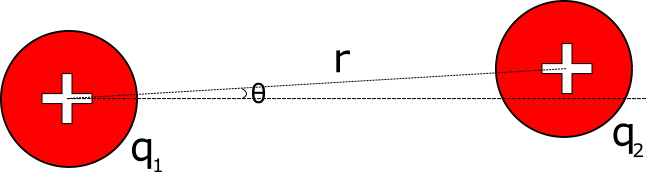
\includegraphics[width=0.8\textwidth]{lab0-session2}
\caption{Setup for the data of Session 2. Two charges $q_1$ and $q_2$ are separated by a distance $r$, and at an angle $\theta$ with respect to some axis horizontal to $q_1$.}
\label{Fig:lab0-session2-setup}
\end{figure}

Given this dataset, you must find how the electric force on $q_1$ is affected by the following parameters:
\begin{itemize}
\item Charges $q_1$ and $q_2$.
\item Distance $r$ between the charges.
\item The angle $\theta$ with respect to a horizontal axis separating $q_1$ from $q_2$.
\end{itemize}

You are given a .txt files from which you are to import them into Excel. For all the .txt files, the charges are in Coulomb units, the forces are in Newton, the angle is in radians and the distance is in meters. \anhkhoi{Change .txt files to have the constant variables and the standard deviations.}

We suggest that you start your analysis for fixed $r, \theta$, but varying $q_1$ and $q_2$. Find how the force $F$ depends on $q_1$ and $q_2$. Support your conclusion by performing appropriate fits to your equation and comparing them to the error bars. If you find that you can simplify their dependence by eq.~\eqref{Eq:f=xy} or \eqref{Eq:f=1/x}, perform the appropriate error propagation equation to find the effective error of this composite quantity.

After you have found the appropriate $q_1$ and $q_2$ dependence, find the dependence on $\theta$ by using appropriate data analysis techniques.

Finally, find the appropriate dependence on $r$. Note that you have 3 different trials for this experiment: you must analyse all three and compare your findings to see if your analysis is self-consistent.

After analysing the effect of the all previous variables, state the equation of the electric force $F(q_1,q_2,r,\theta)$ that best matches your findings. 

Given your equation, what happens if the radius $r$ is much larger or smaller than $q1$ and $q_2$? Is this what you expect physically to occur?

Your methodology can only find the dependence on the explicit variables that you analyse, but the physics can be shifted by an overall constant:
\begin{equation}
F(q_1, q_2, r, \theta) = k \times  f(q_1,q_2,r,\theta) +c.
\end{equation}
What is the significance of $c$? Given all your previous datasets, find the constant factor $k$. If you found the right dependence on your variables, this constant should be the same for all your datasets.

\chapter{Capacitance}
\section{Learning objectives}
\begin{itemize}
\item How to acquire data
\item How to quantify error
\item How to present data
\item Learn about linear fits
\item Confirm capacitance law
\end{itemize}


\section{Introduction}
In this lab you will be asked to accomplish the following tasks:
\begin{itemize}
\item Find possible parameters that could affect the capacitance of a parallel plate capacitor system.
\item Support your conclusion based on a quantitative evaluation of your data.
\end{itemize}

You will have to chose some parameters and quantify their affect on the capacitance of the setup. In the process, you will learn how to acquire good data and how to quantify and present your data. We would like to re-emphasize that collaborations and discussions are encouraged and expected throughout the two sessions.

\begin{tcolorbox}[title=Role as a TA]
Your role as a TA will be to guide them through the ``script" that we present in the protocol section. You should guide them by asking questions and making them think about their results as opposed to giving them the right answer immediately. You will also be required to bring teams together to collaborate with each other. You should clarify the grading method, and re-emphasize that the major part of their grade comes from the log book.
\end{tcolorbox}

In the first session, you will work together to find possible parameters that can affect the capacitance of a pair of parallel plates. Measurements at this stage may be crude; do not worry about that, we are {\it not} evaluating the goodness of the data at this stage, rather the process of thinking about what this data {\it means}, and your thinking process about how to improve your experiment to obtain better data.

During the second session, you will be asked to obtain quantitatively improved data and to compare it with data from the previous session. You must conclude, based on a quantitative evaluation of your data, whether or not, and how, your chosen parameter affects the capacitance of a parallel plate capacitor.


\subsection{Pre-lab activity}
To answer some of these questions, we encourage you to read the \textbf{Data Analysis} chapter of the lab manual.
\begin{enumerate}
\item What is a measurement? Give your own definition of what constitutes a measurement based on your previous courses with lab components (biology, chemistry, physics).
\begin{tcolorbox}[title=Answer]
This is more open-ended. Measurements can be taught of as quantifying observations. Measurements must come with an inherent uncertainty.
\end{tcolorbox}
\item Two engineers must measure the distance between the McGill metro station to the athletic centre to build an underground tunnel. One engineer finds that the distance is $9134 \pm 5$m while the other finds that the distance is $(915 \pm 2) \times 10^1$m. In what ways can they compare their measurements? Do their measurements agree? Explain.
\begin{tcolorbox}[title=Answer]
They should compare the standard deviations to conclude that the measurements of the two engineers agree.
\end{tcolorbox}
\item The city considers to build a metro line between McGill station and the station at University of Montreal. To do this, an engineer decides to use a km-long ruler whose smallest divider is a meter. She \textit{did not} use any other measuring devices. She takes her measurements and presents her findings to her team as $3653.4500$m. What is the uncertainty on this measurement? Did she present enough, too little or too many digits about her measurement? Why?
\begin{tcolorbox}[title=Answer]
The correct way to present this measurement is $3653 \pm 1$m since the smallest increment on her measuring instrument is a meter. She presented too many digits since her measuring tool cannot give such precision.
\end{tcolorbox}
\item Two groups of researchers are trying to test their new methodology to measure the speed of light $c$. Current data shows that the speed of light is roughly $c=2.99 792 \times 10^8$ m/s. The first group finds that $c=2.88 \pm 0.02 \times 10^8$ m/s while the second group finds that $c=3.0 \pm 0.2 \times 10^8$ m/s. What do these measurements tell you about their methodology? What type of mistake may have caused the discrepancy in the first group's results?
\begin{tcolorbox}[title=Answer]
These measurements show that the first group has a more \textbf{precise} methodology, while the second team has a more \textbf{accurate} one. The first group probably has a \textbf{systematic error} that causes this offset.
\end{tcolorbox}
\item How do you know if an experimental result is acceptable and trustworthy? What gives you confidence that your data is trustworthy?
\begin{tcolorbox}[title=Answer]
They should say something about the standard deviation and fit coefficient of determination. Ideally, they would mention that the methodology must be questioned as well.
\end{tcolorbox}
\end{enumerate}

\subsection{What is a capacitor?}
You have learned in class that charges can attract and repel each other. This is because point charges source \textit{electric fields} that apply a force on a test charge. Since there can exist a force between two point charges, there exists a \textit{potential energy} between two point charges $\Delta U$ due to this force. We define the \textit{electrical potential} as \textit{the potential energy change \underline{per unit charge}} as
\begin{equation}
\Delta V = \frac{\Delta U}{q}
\label{Eq:ElectricPotential}
\end{equation}
where $q$ is the \textit{test particle's charge}. In practice, it is more useful to define an electrical potential difference to move \textit{\underline{any} test charge} $q$ from $r=\infty$ to a distance $R$ from a source charge $Q$ as
\begin{equation}
V = \frac{k Q}{R}
\label{Eq:ElectricPotential_point}
\end{equation}
where $k$ is Coulomb's constant $k = {1}/{4\pi \epsilon_0}$. This will have units of \textit{voltage} V. This process is depicted in Fig. \ref{Fig:ElectricPotential_point}.
\begin{figure}[h]
\centering
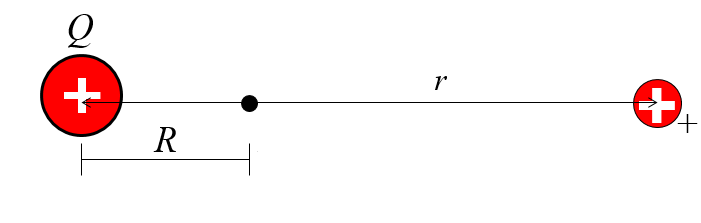
\includegraphics[width=0.7 \textwidth]{lab1-electric-potential.png}
\caption{The electrical potential due to a source charge $Q$ (left) at a distance $R$. The test charge (right) is placed at a distance $r$ from the location that we measure the electrical potential difference.}
\label{Fig:ElectricPotential_point}
\end{figure}

Now consider a pair of parallel plates separated by a distance $d$ connected to a battery as shown in Fig.~\ref{Fig:ParallelPlates}. A pair of parallel plates separated by air or another material can be assembled into a \textit{capacitor}: on each parallel plate, because of the battery, there will accumulate a number of electrons on the negative plate such that the total charge is $-Q$ and $+Q$ on the positive plate. Because of the gap between the plates, there now exists an electric potential between the plates, which is given by eq.~\eqref{Eq:ElectricPotential}.
\begin{figure}[h]
\centering
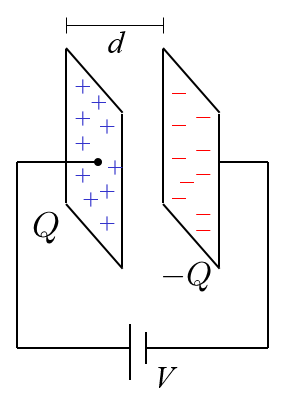
\includegraphics[scale=0.6]{lab1-parallel-plates.png}
\caption{Parallel plate setup. The battery with voltage $V$ creates a flow of electrons such that there will accumulate a total charge of $-Q$ on one plate, and $+Q$ on the positive plate. Since the plates are separated by a distance $d$, there will be a electrical potential difference between the two plates.}
\label{Fig:ParallelPlates}
\end{figure}

One defines the \textit{capacitance} of a capacitor as the constant of proportionality between the total number of charges $Q$ and the electric potential $V$ stored between the plates, i.e. 
\begin{equation}
Q = C V.
\label{capacitor_formula}
\end{equation}
Capacitance is measured in Farads F. A useful constant in such setup is the \textit{vacuum permittivity} $\epsilon = 8.85 \times 10^{-12}$F/m. In this lab, you will be asked to verify \textit{what} affects the capacitance $C$ of a parallel plate capacitor system.

\begin{tcolorbox}[title=Expected result]
We expect them to find
\begin{equation}
C = \epsilon \frac{A}{d}, \nonumber
\end{equation}
where $\epsilon$ is the \textit{relative} permittivity. They should be able to test the area correlation with the plates given, and the distance one by stacking multiple sheets of dielectric between the plates.
\end{tcolorbox}

\begin{tcolorbox}
We expect them to plot their data and fit a linear regression with standard deviation error bars as shown in Fig.~\ref{Fig:Lab1-results-area}. Knowing the distance between the plates, they can also plot the relative permittivity versus the area, and compare with the mean value of $\epsilon$ to see the consistency of their results as shown in Fig.~\ref{Fig:Lab1-results-area2}.
\end{tcolorbox}

\begin{figure}[h]
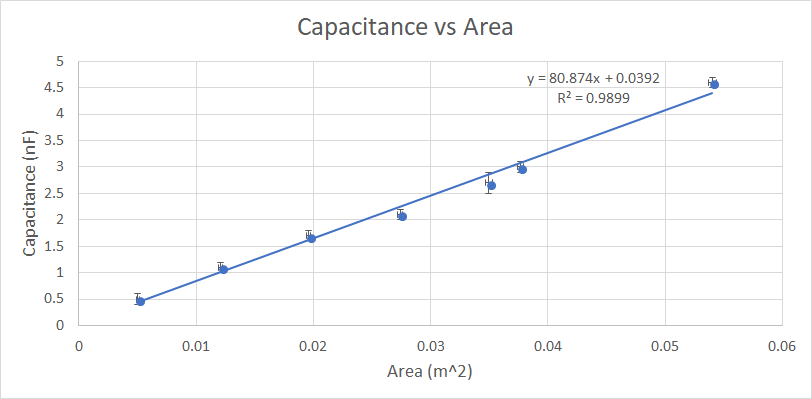
\includegraphics[width=\textwidth]{lab1-results-area}
\caption{[Figure only available to TAs] Data of capacitance versus area. We expect them to display the equation and $R^2$ value. They should be able to find a good linear fit.}
\label{Fig:Lab1-results-area}
\end{figure}
\begin{figure}[h]
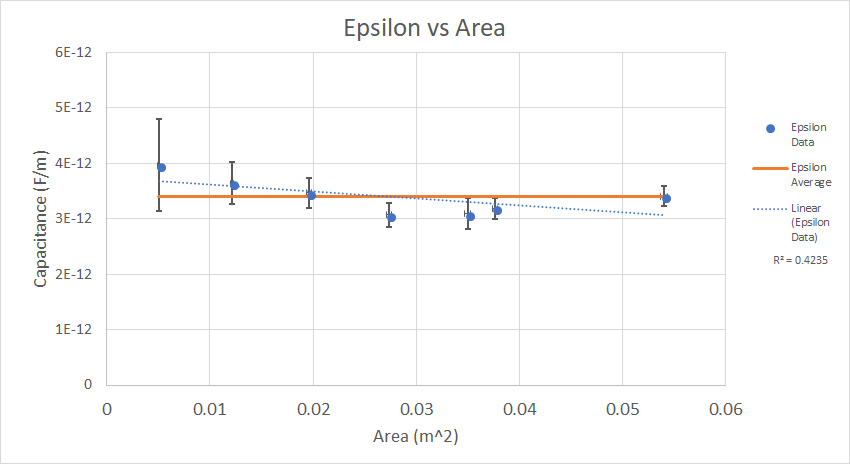
\includegraphics[width=\textwidth]{lab1-results-area2}
\caption{[Figure only available to TAs] Data of the relative permittivity versus the area, compared to the mean value. The average $\epsilon$ is $3.4 \pm 0.3 \times 10^{-12}$ F/m.}
\label{Fig:Lab1-results-area2}
\end{figure}
\begin{figure}[h]
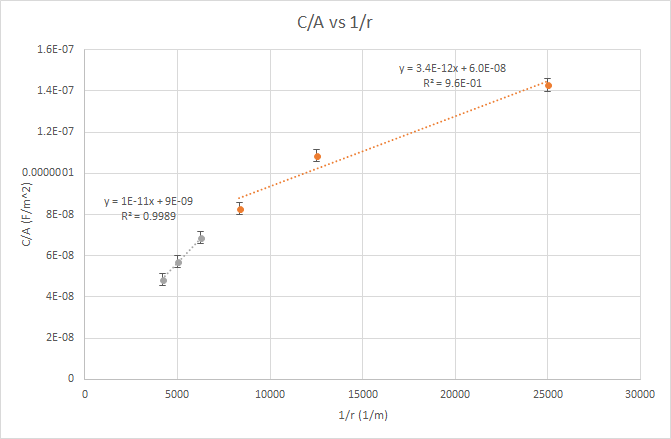
\includegraphics[width=\textwidth]{lab1-results-distance}
\caption{[Figure only available to TAs] Data of $C/A$ versus $1/r$. The data points in orange are those of the first three layers. The linear fit matches the average $\epsilon$ found from the area experiment.}
\label{Fig:Lab1-results-distance}
\end{figure}

\begin{tcolorbox}
When testing for the $d$ dependence, the data showed that for $n>3$ sheets, there seems to be a $1/\sqrt{d}$ correction that appears, and therefore students aren't expected to find a perfect fit for large distances of $d$. This is mostly due to some polarization effect from stacking the dielectrics, and therefore one should view the $1/d$ dependence as a ``small distance" approximation. You should encourage students to find this disparity between experiment and theory and encourage them to discuss the cause of this. The data is shown in Fig.~\ref{Fig:Lab1-results-distance}.
\end{tcolorbox}

\begin{tcolorbox}
Students are encouraged to discuss about other parameters such as shape, volume, mass applied to the dielectric, and the use of other dielectrics, but these aren't easily quantifiable parameters.
\end{tcolorbox}

%\begin{equation}
%C = \epsilon \frac{A}{d}, \qquad \epsilon = \kappa \epsilon_0
%\end{equation}


\section{Protocol}
\subsection{Session a}
\begin{tcolorbox}[title=Session \#1]
We suggest the following time distribution for this session:\\

During the first 20mins, assemble everyone to the front and do a quick introduction, and maybe a demo of the manipulations. You should then ask everyone what they think could affect the capacitance of a capacitor, and push them to give a physical reason behind their hypotheses. We expect you to motivate the idea that electrical potential is given by the relative distance between two charged objects, and therefore, for parallel conducting plates, larger area would allow for more charges to accumulate, and by eq.~\eqref{Eq:ElectricPotential_point}, we expect there to be a $1/r$ dependence. Recommend that they works together to cover more parameters e.g. one team takes care of area, the other does distance.
\end{tcolorbox}

\begin{tcolorbox}
Give them about 60-75mins to perform their measurements while walking around, answering questions and facilitating discussions between teams and teammates. During this period, make sure that everyone makes at least three measurements of varying area with the two plates perfectly aligned. This will serve as a baseline to put them on the right track. Also, do not forget to verify that students have done their pre-labs.
\end{tcolorbox}

\begin{tcolorbox}
After about 90mins of the 2-hour session, call everyone to the front and ask people to describe their findings. List on the board what could affect capacitance and why. Make sure that they support their findings with statistics (standard deviations and fits), and ask them whether the correlations that they find are well supported and warrant extra verification during the next session. After this discussion period, make sure that everyone understands that they have to be looking to verify the effects of area and distance of the plates during the next session.
\end{tcolorbox}

\begin{tcolorbox}
For the remainder of the time, students can try and take additional measurements, and prepare notes for the next session. Don't forget to pick up every teams' log book by the end of the session.
\end{tcolorbox}

The available material is listed in Table \ref{Tab:Lab1-material}. The metallic rectangular plates will be of varying dimensions. The manipulations are straightforward: insert either a plastic or paper sheet between the two plates and use the Arduino unit (see below) to measure the capacitance. At this point, you do not need to know how the Arduino unit works, simply how to use it. You will learn how it works in the next lab. The plates must not touch each other in order for you to see a measurement: this causes a short-circuit and therefore you will not see a capacitance measurement. You can assume that the distance between the plates is the thickness of the plastic or paper sheet.
\begin{table}[h]
\centering
\begin{tabular}{||c | c ||}
\hline
Individual station & Collective station\\ \hline
Laptop & Aluminum foil \\
Arduino capacitance setup & Blocks of wood \\
Metallic plates & Small weights \\
Ruler (?) & Assorted capacitors \\
Plastic sheets & Assorted resistors \\
Paper sheets & Extra wires \\
& Micrometer \\
& Multimeter \\
\hline
\end{tabular}
\caption{Available material for Lab \# 1}
\label{Tab:Lab1-material}
\end{table}

\noindent Information about the Arduino code can be found \href{https://www.arduino.cc/en/Tutorial/CapacitanceMeter}{here}. To use the Arduino unit:
\begin{enumerate}
\item Plug the USB-port into the laptop
\item Open the Arduino Genuino application on the laptop.
\item Open the capacitanceMeter.ino file found in \anhkhoi{location}.

\item In the tabs above, go into the drop-down menu Tools $\rightarrow$ Port. Choose whichever COM is labelled by ``(Arduino/Genuino Uno)".
\begin{figure}[H]
\centering
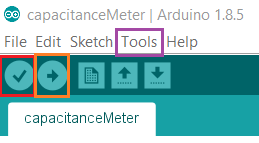
\includegraphics[width=0.5 \textwidth]{lab1-Arduino-menu-bar.png}
\caption{Arduino application menu bar. Note that the color boxes were added manually. The red checkmark box is the \textbf{verify} button. It serves to verify whether there is an error in the code. The orange right arrow box is the \textbf{upload} button, and the purple box is the \textbf{Tools} drop-down menu bar.}
\label{Fig:ArduinoMenuBar}
\end{figure}

\item Verify the script by clicking the icon with a checkmark. If there is an error, call the TA.
\item Upload the script by clicking the icon with the right arrow.
\item In the tabs above, go into Tools $\rightarrow$ Serial Monitor (or on your keyboard, press Ctrl+Shift+M).
\begin{figure}[h]
\centering
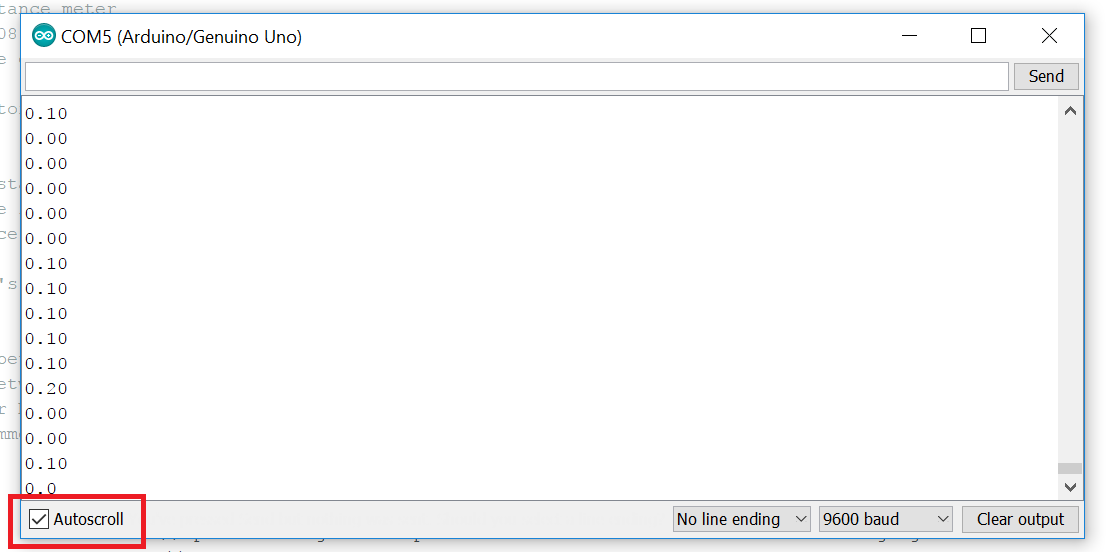
\includegraphics[width=0.85 \textwidth]{lab1-Arduino-monitor.png}
\caption{Arduino Serial Monitor. This is a pop-up screen where you will see your capacitance measurements scroll by. The Arduino unit takes a capcitance measurement at a fixed frequency. Unless otherwise specified, the output is in nanoFarads. Units aren't display as to simplify the transfer from the monitor screen to Excel, but one could display the units by changing the command in the Arduino script. To stop the scrolling of measurements, click on the Autoscroll box.}
\label{Fig:Arduino-Monitor}
\end{figure}

\item Take the two wires (see Fig.~\anhkhoi{updated setup}) and simply touch each side of the parallel plates: you should see a multitude of measurements scrolling down the monitor window. If you do not see many measurements scrolling in the monitor window, it is likely that the plates are touching each other. \anhkhoi{input new setup pic}
\item You can stop the auto-scroll by clicking the bottom-left box to better see your results (see Fig.~\ref{Fig:Arduino-Monitor}).
\end{enumerate}

Notice that in Fig.~\ref{Fig:Arduino-Monitor}, the data fluctuates. You will have to determine how many capacitance measurements should you average over to acquire a good representation of that capacitance measurement. We refer you to the ``\textbf{Error Analysis}" section of the lab manual. Using this setup, proceed to conduct you experiments and collect data that will let you evaluate $C$ in in eq.~\ref{capacitor_formula}. 

You will have the opportunity to test whatever hypothesis you may have, however \textbf{every group must take a capacitance measurement for at least \underline{three} different pairs of plate sizes while inserting a single sheet of plastic between them. The plates must be perfectly aligned on top of each other}. After doing so, you may explore in more details the consequences of these measurements, or you may study other possible parameters that could affect the capacitance.

\begin{tcolorbox}
The three area measurements will serve as a baseline for students in case some of them attempt to test unconventional hypotheses.
\end{tcolorbox}

Given the measurement of the two sides $L_1$ and $L_2$ of a rectangle and their corresponding standard deviations $\sigma_{L_1}$ and $\sigma_{L_2}$, the standard deviation on the area is given by
\begin{equation}
\sigma_A = \sqrt{ \left( L_1 \sigma_{L_2} \right)^2 + \left( L_2 \sigma_{L_1} \right)^2 }.
\end{equation}

While studying other parameters, if you are unsure of the standard deviation of a certain parameter, you may ask the TAs to derive the appropriate derived standard deviation for that parameter.

Enter your set up, measurement process and data in your log book. Before handing in your log book, be sure to write down your observations in the \textbf{General Notes} section of your log book, and a rough plan of what you intend to do during the next session in the \textbf{Conclusions and future work} section. The latter part should be done after discussions with at least one other group. You \textbf{do not need to include a results section} in your log book for this session.

\subsection{Session b}
We recommend that you bring whatever material that you think could help you acquire better data. At this point, you should know what parameters affect the capacitance, and therefore you should plan in advance your own ``protocol" to verify your hypothesis quantitatively with improved data. This protocol does \underline{not} have to match what you wrote in your log book during the last session, but if it does differ, you must explain what made you change your mind.

\begin{tcolorbox}[title=Session \#2]
In this session, you should remind everyone that last time, you discovered together that $C \propto A/d$, so this session should be simpler as they will know what to do.
\end{tcolorbox}

Be mindful that you will be evaluated based on your data presentation, data analysis and explanation of the physics, therefore be certain to \textit{fully, but succinctly, describe} your thought process. 

\section{Measurement Analysis}
During this lab, you will have to use data analysis techniques to understand your data. For \underline{each session}, we recommend that you analyse your data as follows.

To study a system, one typically isolates as many variables as possible to see each of its individual affect on the whole system. If we are able to isolate such a variable, mathematically, that is the equivalent of finding some $f(x)$ that depends just on one variable $x$. In this lab, you will find as many variables that can affect the capacitance as possible by isolating each parameter one at a time.

For each dataset, corresponding to each parameter you measure, you must abide by the error analysis rules outlined in the first part of the lab manual. The data analysis can be done much more rapidly with spreadsheets, therefore we highly recommend that you read that section (\textbf{Introduction to Excel}) which can be found in the appendix of the lab manual. When analysing your data, you must follow the norms established in the \textbf{Data Analysis} chapter to understand the significance of your data. 

Once you have some result from your data, you must offer a physical explanation that supports your results. Explain why physically each parameter affects the capacitance of the system. Support your claim by proposing a possible experiment to test your claims, and offer possible outcomes that one could observe from your experiment. Recall that bouncing your ideas off peers is an invaluable way to actually test the rational of your hypothesis.


\chapter{RC Circuits}
\section{Learning objectives}
\begin{itemize}
\item Learn how to connect circuits
\item Learn about exponential functions
\item Learn about RC circuits
\item Learn about equivalent resistance and capacitance
\end{itemize}

\section{Introduction}
In this lab you will characterize an RC circuit. An RC circuit is a circuit that contains a resistor (R) and a capacitor (C). The analysis tool we will use is called a PASCO 850 Universal Interface, the use of which will be explained below. Specifically, we will also use a voltmeter and a
signal generator tool to examine the charging and discharging of a capacitor. 

In the first session, you will be asked to \textbf{measure the time constant} of a given RC circuit. In the process, you will learn how to measure time constants and understand subtleties in the data acquisition apparatus. This session will be a more traditional lab where you will follow well outlined instructions. 

In the second session, you will be asked to \textbf{build an RC circuit with a specific time constant} and to show, based on well supported data, that your circuit has the appropriate time constant. When you arrive at the second session, you will receive a sheet that asks you to build an RC circuit with a specific number of parallel branches. You are to choose an appropriate number of resistors and capacitors to obtain a specific time constant.

\subsection{Pre-lab activity}
\begin{enumerate}
\item Why would we want to fit a dataset to an equation?
\begin{tcolorbox}[title=Answer]
Curve fitting allows one to match data to a quantitative theoretical model. A good model is able to predict future outcomes of similar experiments.
\end{tcolorbox}
\item What is $e^{x}$ evaluated at $x=0$, $x=1$ and $x=-1$?
\item For $f(x) = e^{-x}$, what is the value of $x$ so that $f(x)=0$?
\item What does $a$, $b$ and $c$ do in the following function?
\begin{equation}
f(x) = a e^{b x}+c
\end{equation}
\item What is the difference between these two plots:
\begin{figure}[h]
\centering
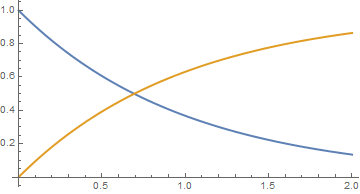
\includegraphics[width=0.7\linewidth]{lab2-prelab}
\caption{Exponential functions.}
\label{Fig:lab2-prelab}
\end{figure}
\end{enumerate}

\subsection{RC Circuits}
Recall that the capacitance is defined as the proportionality constant between the total charge accumulated by a capacitor and the voltage across the circuit
\begin{equation}
Q = C \Delta V.
\end{equation}
In this equation, the charge $Q$ is expressed in Coulomb (C), the voltage $\Delta V$, in volts (V) and the capacitance $C$ in farads (F).

In this lab you will study both the \textit{charging} and \textit{discharging} process of an RC circuit. During the charging process, charges accumulate on each sides of the parallel plate capacitor. During the discharging process, the capacitor releases all its charges into the circuit. Capacitors charge and discharge exponentially in time. During the \textit{discharge} of a capacitor, the instantaneous voltage $\Delta V_C$ between the ends of the capacitor also drops and is given by
\begin{equation}
\Delta V_C = \Delta V_{max} e^{-t/\tau}
\label{Eq:V-discharge}
\end{equation}
where $\Delta V_{max}$ is the maximum voltage across the capacitor, i.e. the voltage to which the capacitor was charges, $t$ is the time and $\tau$ is the \textit{time constant} given by
\begin{equation}
\tau = R_{eq} C_{eq}
\label{Eq:time-constant}
\end{equation}
where $R_{eq}$ and $C_{eq}$ are respectively the equivalent resistance and capacitance of the circuit. Although the theoretical discharge time is infinite, in practice we consider that the discharge is over when the voltage at the bounds of the capacitor is at $1\%$ of its maximal value. 

\subsection{Equivalent resistance and capacitance}
To find the equivalent resistance and capacitance of a circuit, one must apply the correct equations to sum the contributions of all the components.. The equivalent quantity differs depending on whether the resistors and capacitors are combined in series or in parallel. For resistors, the equivalent resistance is given as
\begin{equation}
R_{series} = R_1 + R_2 + R_3 + ... R_n = \displaystyle \sum_{i=1}^n R_i
\end{equation}
\begin{equation}
\frac{1}{R_{parallel}} = \frac{1}{R_1} + \frac{1}{R_2} + \frac{1}{R_3} + ... + \frac{1}{R_n} = \displaystyle \sum_{i=1}^n \frac{1}{R_i}
\end{equation}

For capacitors, the equivalent capacitance is given as
\begin{equation}
C_{parallel} = C_1 + C_2 + C_3 + ... C_n = \displaystyle \sum_{i=1}^n C_i
\end{equation}
\begin{equation}
\frac{1}{C_{series}} =  \frac{1}{C_1} + \frac{1}{C_2} + \frac{1}{C_3} + ... + \frac{1}{C_n} = \displaystyle  \sum_{i=1}^n \frac{1}{C_i}
\end{equation}

\subsection{Equipment} \label{Sect:lab2-equipment}
In this lab you will use the PASCO 850 Universal Interface to measure and plot voltages as a function of time in an RC circuit. The PASCO devices comes with two sets of wires (see Fig.~\ref{Fig:lab2-PASCO}). The first is the input/output voltage source. The other is a set of probe which measures the voltage across the capacitor of the circuit. 

\begin{figure}[h]
\centering
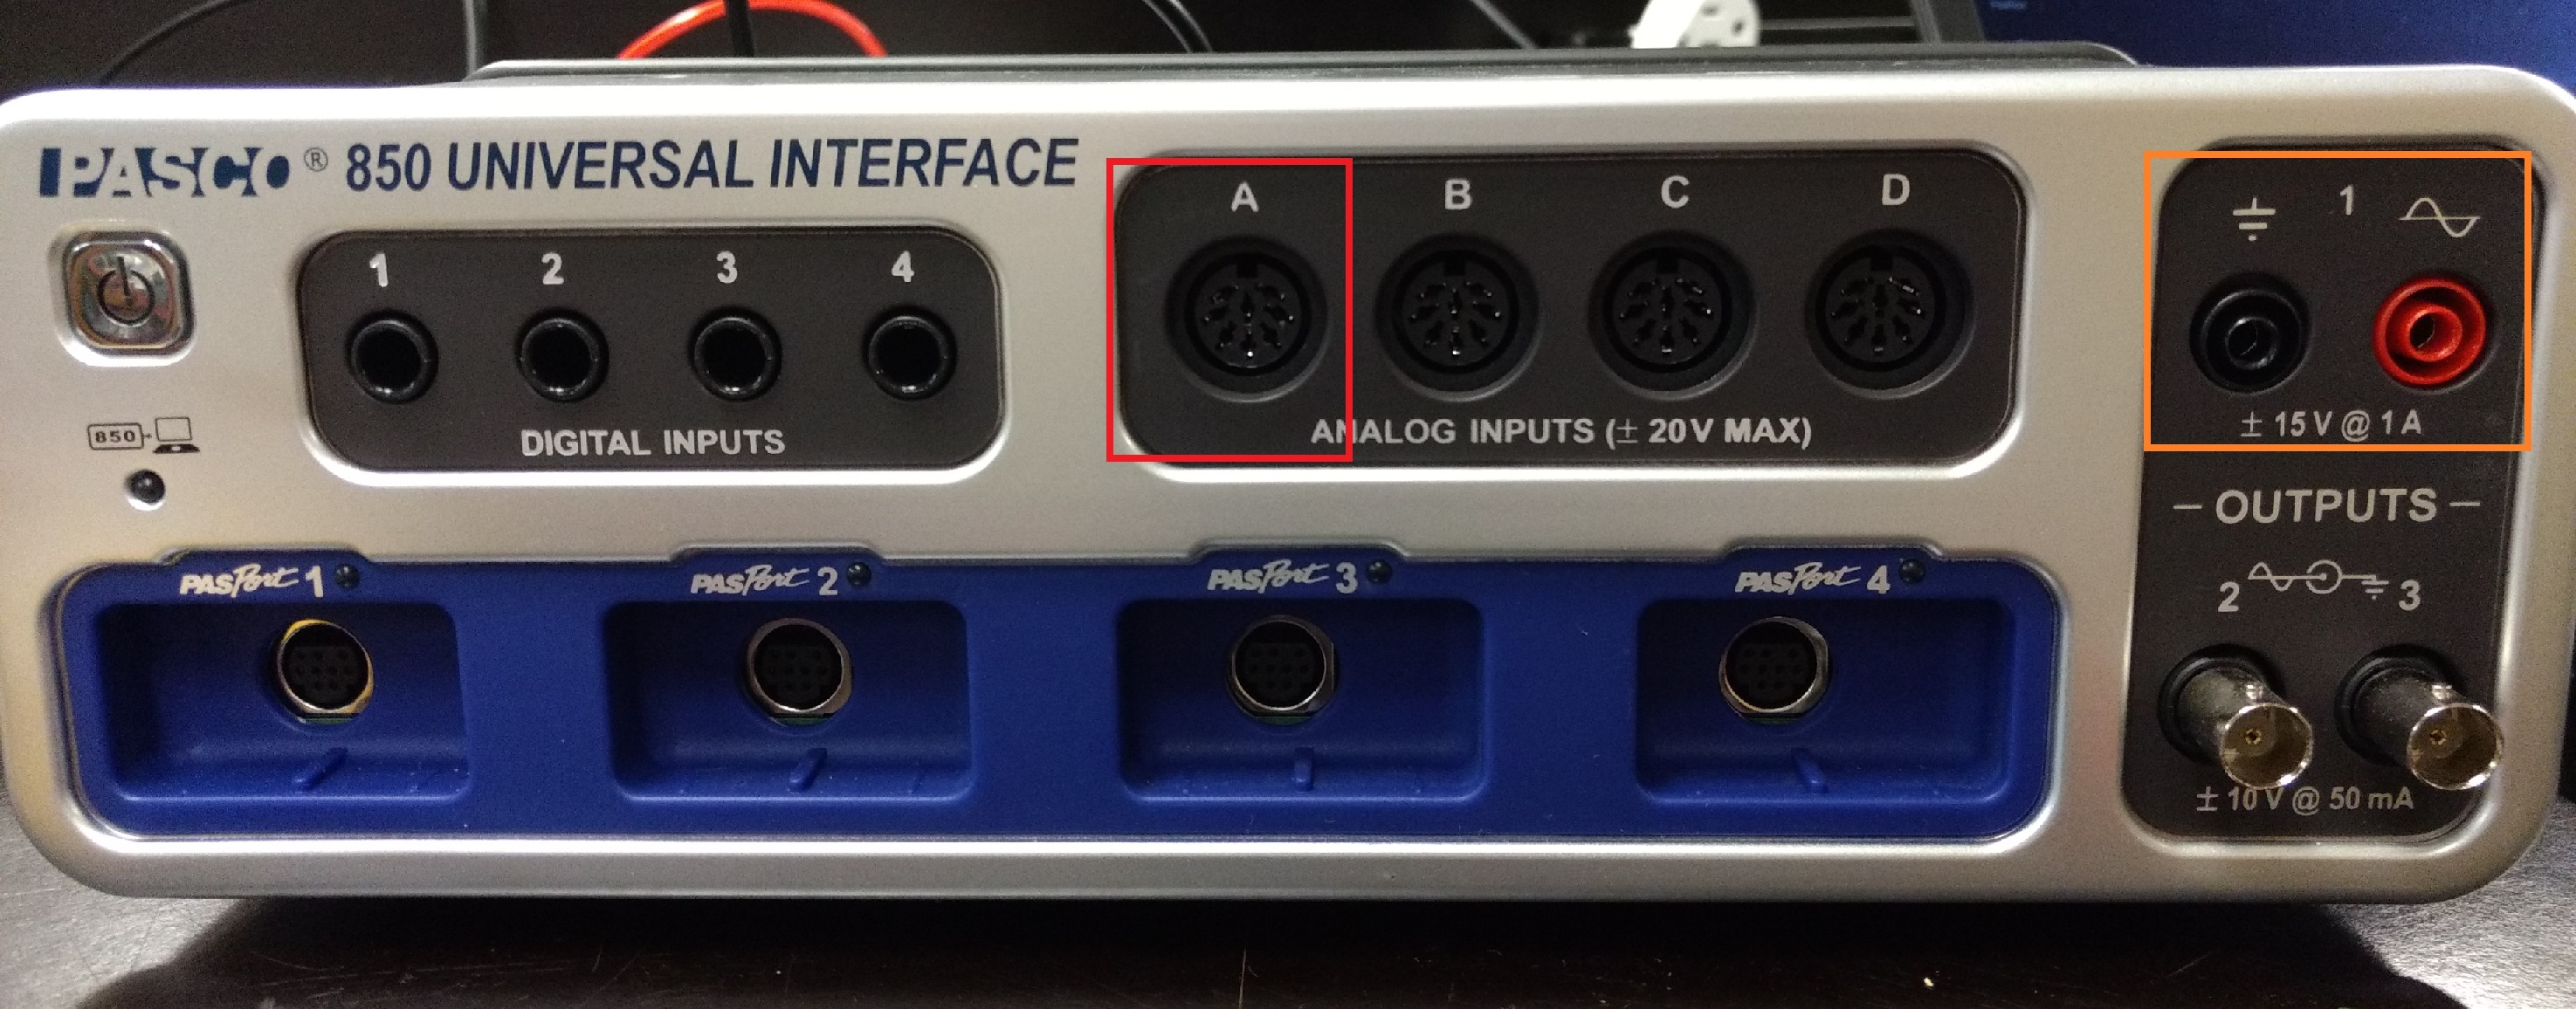
\includegraphics[width=0.8\linewidth]{lab2-PASCO}
\caption{PASCO 850 Universal Interface The red box is the probe Analog input. The voltage source (Output 1) is boxed in orange.}
\label{Fig:lab2-PASCO}
\end{figure}

Given the nature on these measurements, there is an inherent fluctuation to the data that is difficult to characterize. During the first session, you are not required to produce quantitatively well supported data. But for the second session, you are to demonstrate that you've produced an RC circuit with the correct time constant. 
%Therefore the following standard deviation rules for PASCO measurements have been adjusted (and tested) to time constants of this second session. This is to compensate for the fluctuation of the voltage measurements.

%For time difference measurements, the standard deviation will be $\sigma_t = 10^{-4} s$. To convert the error from the Curve fitting parameter $B$ to the time constant $\tau$, based on eq.~\eqref{Eq:1/x error}, one must take
%\begin{equation}
%\sigma_\tau = 100 \frac{\sigma_B}{B^2} \text{s}.
%\label{Eq:lab2-error-tau-fit}
%\end{equation}
%The factor of $100$ was found to appropriately adjust for voltage fluctuations.

\section{Session a}
\noindent \large \textbf{Equipment} \normalsize \\
During the first session, you will receive an RC circuit fastened onto a wooded board. Before proceeding with measurements related to charging and discharging capacitors, conduct the following steps:
\begin{enumerate}
\item Turn the wooden board over to reveal the circuit Fig.~\ref{Fig:lab2-session1-circuit1}. There are actually two circuits here, one consisting of a $100$k$\Omega$ rheostat (variable resistor) and the $100\mu$F capacitor, the other consisting of a $470\Omega$ resistor and a $0.1\mu$F capacitor. We will not use the $0.1 \mu$F capacitor, or the rheostat.
\item Connect the Output 1 of the PASCO 850 Universal Interface to the wooden board's terminals as well as the Analog Input A in order to complete the circuit as shown on Fig.~\ref{Fig:lab2-session1-circuit1}. The $100\mu$F capacitor can now charge through the $470\Omega$ resistor (when in the ``charge" state) and discharge through the $150$k$\Omega$ resistor (when in the ``discharge" state). The charging voltage is read on the computer. The Input A measures the voltage through the 100$\mu$F capacitor. The Output 1 is the one with the red and black connectors and the analog inputs are the higher half of the interface and on the right.
\end{enumerate}

\begin{figure}[h]
\centering
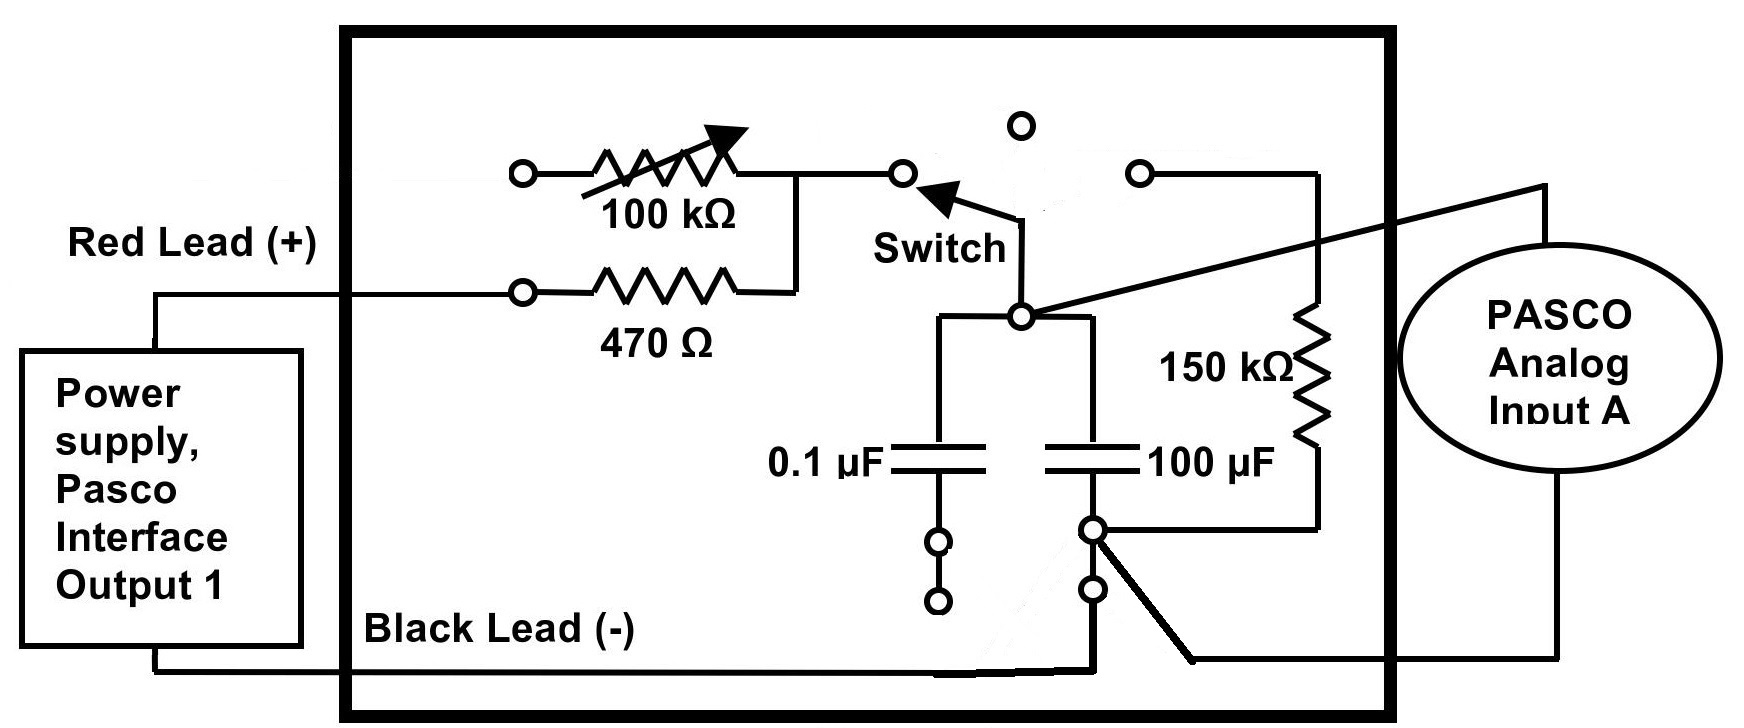
\includegraphics[width=0.75\linewidth]{lab2-session1-circuit2}
\caption{Circuit for session 1. This is currently connected to the rheostat.}
\label{Fig:lab2-session1-circuit1}
\end{figure}

\begin{tcolorbox}[title=Session \#1]
In this session you will supervise students as they perform the protocol below. You may gather students in the beginning to give a brief introduction and summary of the lab. By the end, they should be comfortable measuring charging/discharging time constants. When they use the square wave input, make sure that they understand how to vary the parameters to obtain good data, i.e. changing the frequency of the function generator and the frequency of data acquisition.
\end{tcolorbox}

\noindent \large \textbf{Procedure} \normalsize \\
You will execute the following steps in order to understand how to use the PASCO interface to characterize an RC circuit. For this session, you are expected to write down your observations in your log book and to answer the questions that appear in the following instructions. You should write down all that technical notes about the apparatus and how an RC circuit works in order for you to fast-track your manipulations for the next session.
\begin{enumerate}
\item Connect the circuit as shown in Fig.~\ref{Fig:lab2-session1-circuit1}.
\item \anhkhoi{Where to get Pasco file}
\item Turn on the PASCO and plug in the USB into the computer.
%\item On the software, open the ``Signal Generator" tool, which is located on the left hand side panel and make sure that the signal is set to be DC (Waveform option), has an amplitude of $6V$ and has a data acquisition frequency of $10$ Hz. See Fig.~\ref{Fig:lab2-interface-dc}.
%\begin{figure}[h]
%\centering
%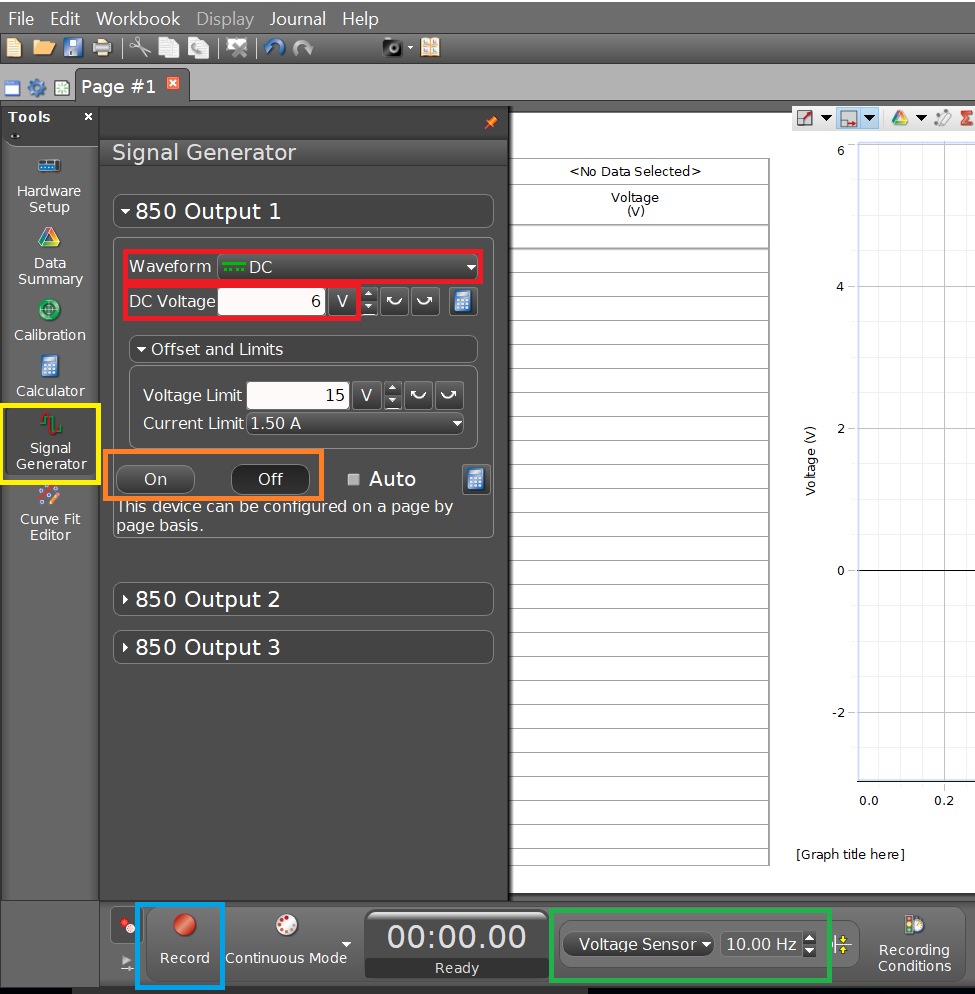
\includegraphics[scale=0.5]{lab2-interface-dc}
%\caption{Settings for a DC waveform input. To find this toolbar, select the ``Signal Generator" tool (yellow box). The red boxes are to set the waveform of the input and the amplitude. Set the data acquisition frequency to 10Hz (see green box). To turn On or Off the signal generator, see the orange box. To record data, select the red recording button (boxed in blue). }
%\label{Fig:lab2-interface-dc}
%\end{figure}

%\item Set the rheostat to its maximum value (turn fully clockwise).
%\item Press the red round Record button, on the bottom panel .
%\item On the computer, under the 850 Output 1, press On to turn on the power supply.
%\item Flip the switch to the ``Charge" position. A graph should slowly appear on your screen. Log the time it takes for the capacitor to charge.
%\item When the capacitor is charged, press the red button that now says Stop.
%\item Press that same button that now says Record and set the switch to discharge the capacitor and notice the rate of the voltage drop. When the capacitor is discharged, stop the recording.
%\item Repeat steps 5 to 8 for the rheostat at approximately half its value and at its minimum value. Compare the charging rates from step 8 (with the maximum rheostat value) with these two new rheostat values. Discuss your qualitative observations in the ``General notes" section of your log book.
%\item Discharge the capacitor (steps 9,10) and record it for the minimum rheostat value. 
%The software can perform an exponential regression on the data you record. To make good use of that, activate the Curve Fitting option (see Fig.~\ref{Fig:lab2-interface-graph}). The curve of eq.~\eqref{Eq:V-discharge} will be fit to the whole data set. To fit it on the right segment on the data set, use the highlighting tool and select/box the values that are most relevant. The time constant is given by the parameter $1/B$ in the curve fitting data window. The error is given by eq.~\eqref{Eq:lab2-error-tau-fit}.
%\begin{figure}[h]
%\centering
%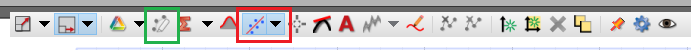
\includegraphics[width=0.9 \linewidth]{lab2-interface-graph-tools}
%\caption{Graphing toolbar. The toolbar appears when moving the mouse to the top of the graph. The red boxed icon is the Curve fitting tool. Select the ``Natural Exponential" function. The highlighting tool is boxed in green. This allows to select a smaller subset of data to apply the curve fitting.}
%\label{Fig:lab2-interface-graph}
%\end{figure}

%\item \textbf{Determine the time constant $\tau$ of the circuit}. $\tau = RC$ is the time the voltage takes to decrease from its maximum value $V_0$ to $1/e$ of $V_0$ (see Section 19.6 of your notes). Use the discharge data from the PASCO in step 12 to determine this. How does the value obtained from the data compare to the fitting exponent provided by the software regression in step 12?
%\item The capacitance value of $100 \mu$F is only approximate. \textbf{Determine} the true capacitance from the time constant measured in step 13 and recalling that $\tau=RC$ (assume that the resistance of $150$k$\Omega$ is correct).
%\item When a capacitor is discharging, the formula is $Q=Q_{max} e^{-t/\tau}$ while when it is charging, the equation is $Q=Q_{max} (1 - e^{-t/\tau})$. What is the difference between the $(1-e^{-x})$ and $e^{-x}$ functions? Explain this in your log book.


%\item We will now learn how to obtain time constants from square wave inputs: we must first connect the 470$\Omega$ resistor in series with the $100\mu$F capacitor as shown below.
%\begin{figure}[h]
%\centering
%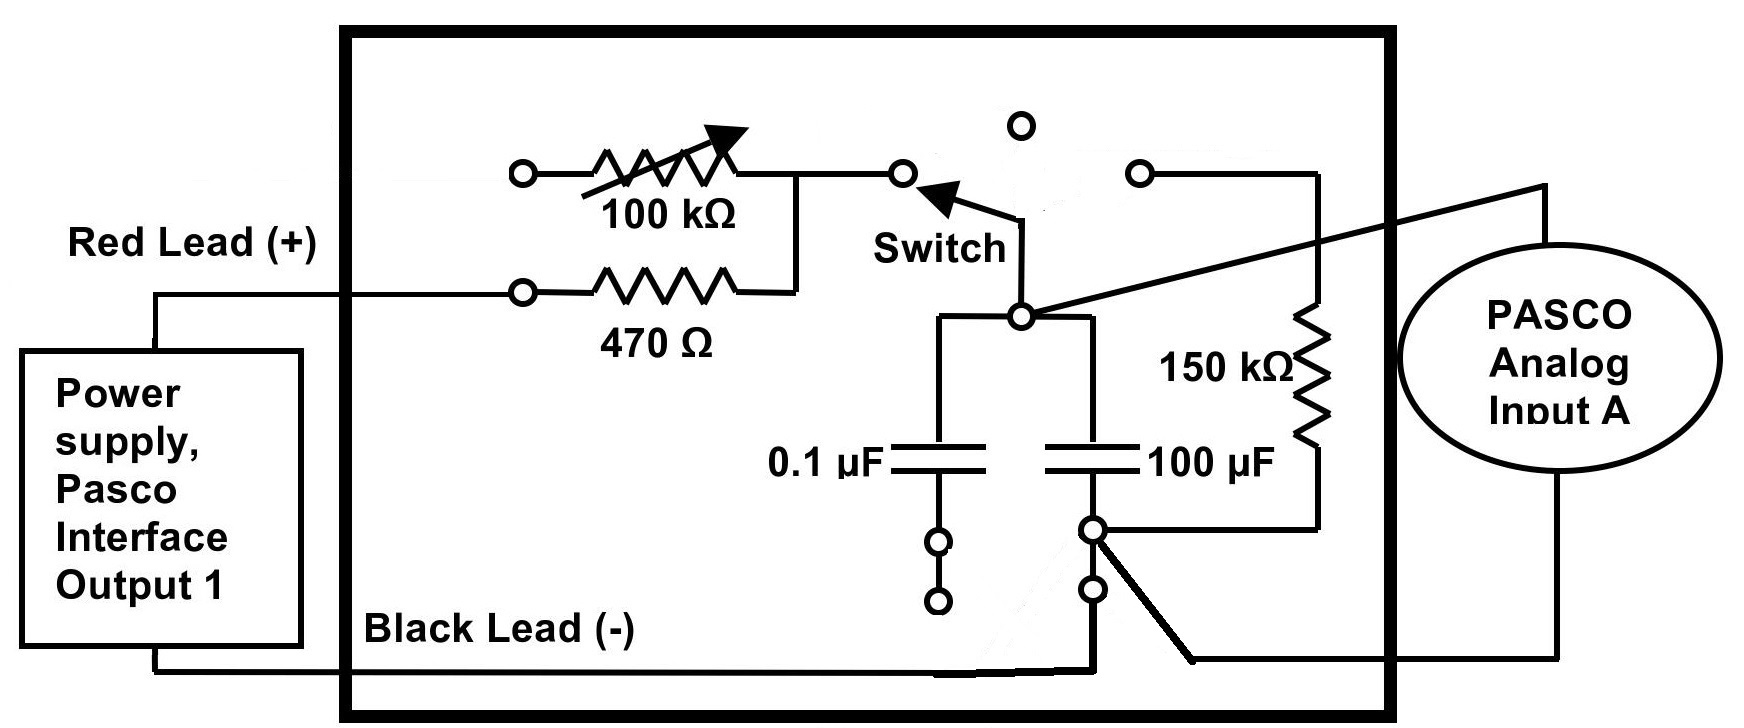
\includegraphics[width=0.75\linewidth]{lab2-session1-circuit2}
%\caption{Connection of the circuit for the $470\Omega$ resistor in series with the $100\mu$F capacitor. By leaving the switch at the position shown, both charging and discharging constants should be the same.}
%\label{Fig:lab2-session1-circuit2}
%\end{figure}

\item In the software, open the ``Signal Generator" tool, which is located on the left hand side panel and make sure that the signal is set to "Positive Square Wave" with an amplitude of 6V and frequency of 0.5 Hz. This is equivalent turning on and off a DC voltage 2 times per second. Change the data acquisition frequency found at the bottom of the interface to $1$kHz. See Fig.~\ref{Fig:lab2-interface-square-wave}.
\begin{figure}[h]
\centering
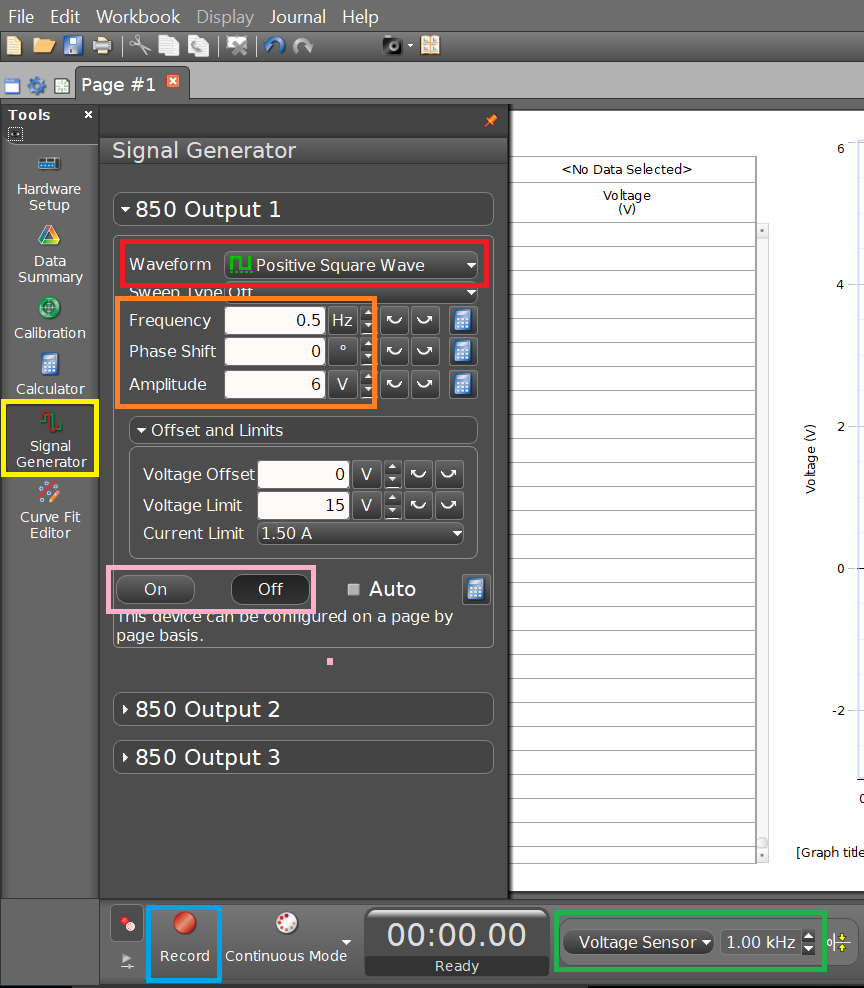
\includegraphics[scale=0.5]{lab2-interface-square-wave}
\caption{Settings for a positive square wave input. You must first select the ``Signal Generator" setting in the yellow box. The red box allows to change the waveform. Change the frequency and amplitude according to the orange box. Change the data acquisition frequency to the values in the green box. Once you are ready to record your data, select the record button (blue box), and turn on the voltage source (pink box)}
\label{Fig:lab2-interface-square-wave}
\end{figure}

\item With this input from the "Signal Generator" you won't use the "charge" and "discharge" switch from the wooded board. Instead you will simply turn On and Off (pink box) the power supply under the 850 Output 1 panel before and after recording measurements. So leave the switch on ``charge" for the rest of the experiment.
%\item Since your time constant is smaller than what you observed from discharging through the $150$k$\Omega$ resistor, you will not need to record data for long.
\item After turning on the signal generator, press the record button twice to record and stop the recording after observing a few charges/discharges.
\item Zoom in on a region with both charging and discharging behaviours by rescaling the axes, and figure out which section corresponds to charging/discharging.
\item For the charging part, measure the time difference between the moment the voltage starts increasing to the moment where the voltage is at a value $1-1/e$ of the maximum voltage $V_0$. You should understand why you are measuring this time difference.
\item For the discharging part, you will use the Curve fitting tool. The software can perform an exponential regression on the data you record. To make good use of that, activate the Curve Fitting option (see Fig.~\ref{Fig:lab2-interface-graph}). The curve of eq.~\eqref{Eq:V-discharge} will be fit to the whole data set. To fit it on the right segment on the data set, use the highlighting tool and select/box the values that are most relevant. The time constant is given by the parameter $1/B$ in the curve fitting data window.
\begin{figure}[h]
\centering
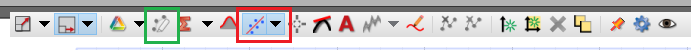
\includegraphics[width=0.9 \linewidth]{lab2-interface-graph-tools}
\caption{Graphing toolbar. The toolbar appears when moving the mouse to the top of the graph. The red boxed icon is the Curve fitting tool. Select the ``Natural Exponential" function. The highlighting tool is boxed in green. This allows to select a smaller subset of data to apply the curve fitting.}
\label{Fig:lab2-interface-graph}
\end{figure}

Use this to fit an exponential curve to the discharging region. You will obtain the discharge time constant.
\item Compare the time constants obtained from both the charging and discharging regions and by keeping track of the standard deviations as mentioned in section~\ref{Sect:lab2-equipment}. Calculate the theoretical time constant based on the known values of resistance and capacitance (see step 14). Recall that the standard deviation of the product of two variables is given by eq.~\eqref{Eq:product error}. Can you explain difference in standard deviation, and why some are smaller/larger than the others? You can repeat steps 6-10 for different segments of charging/discharging in your data if you want to verify the consistency of your measurements.
\item Answer the following questions in the results section of your log book. Should all the time constants be the same or different? Why and why not? What would happen if we had used the rheostat instead of the $470\Omega$ resistor in Fig.~\ref{Fig:lab2-session1-circuit1} and used a DC voltage source (with the On/Off switch on the board) instead of a wavefunction source: would we have the same time constant for both charging and discharging? What would happen to the time constant if we increased the resistance by using the rheostat? If you have time, you should test your hypotheses experimentally.

\begin{tcolorbox}[title=Answer]
All the time constants should be the same because we are charging and discharging across the same resistor. If we had used the rheostat with a DC voltage and the On/Off switch, since we're charging and discharging across different resistors, the time constants should be different. By eq.~\eqref{Eq:time-constant}, the resistance should affect the time constant linearly.
\end{tcolorbox}

\item Answer the following in the results section of your log book. Assuming the voltage, when completely charged, is set to $V_0 = 1$ and by considering the variables $\tau$ for time constant and $t$ for time, what are the equations for of charging and discharging? Support your answer by physical arguments.

\begin{tcolorbox}[title=Answer]
Discharging is $V = e^{-t/\tau}$ and charging goes as $V=1-e^{-t/\tau}$. At $t=0$, we expect the charging function to be $0$ and the discharging function to be $1$. Similarly, at $t\rightarrow \infty$, the reverse must be true.
\end{tcolorbox}

\item Answer the following in the results section of your log book. Your draft calculations can be shown in the ``General Notes" section of the log book. In the circuit of Fig.~\ref{Fig:lab2-session1-Rpractice}, how will the fully charged capacitor affect the current and potential in R6? Answer this in your log book.
\begin{figure}[h]
\centering
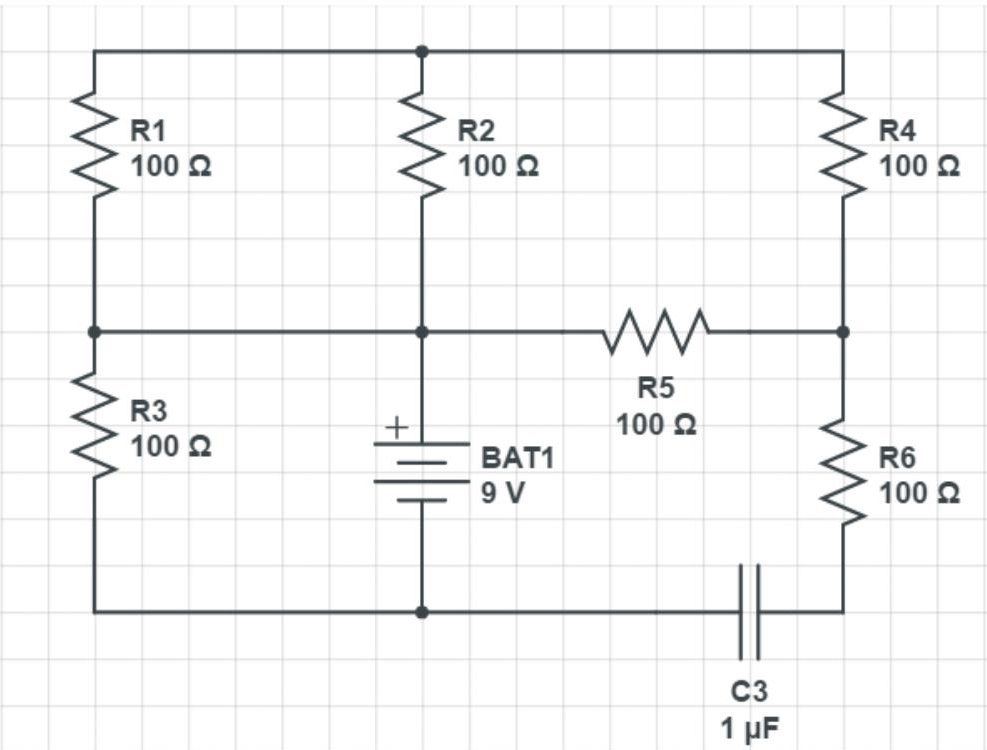
\includegraphics[width=0.6\linewidth]{lab2-session1-Rpractice}
\caption{Effect of a fully charged capacitor on the circuit.}
\label{Fig:lab2-session1-Rpractice}
\end{figure}

\begin{tcolorbox}[title=Answer]
The current is defined as the change in charge over time. In other words,
\begin{equation}
\frac{dQ}{dt} = C \frac{dV}{dt} = I.
\end{equation}
Therefore if the capacitor is fully charged, the change in voltage vanishes and so the current also vanishes: it is then considered like an open-circuit. Thus the potential across R6 vanishes.
\end{tcolorbox}

\item Answer the following in the results section of your log book. Your draft calculations can be shown in the ``General Notes" section of the log book. Given Fig.~\ref{Fig:lab2-session1-tau-practice}, what must be the value of C2 such that the time constant is approximately $\tau=12.5$ms. If one replaces C2 by two capacitors in series, one of which has $C5=250\mu$F. What must be the capacitance of the second capacitor to preserve the same time constant?
\begin{figure}[h]
\centering
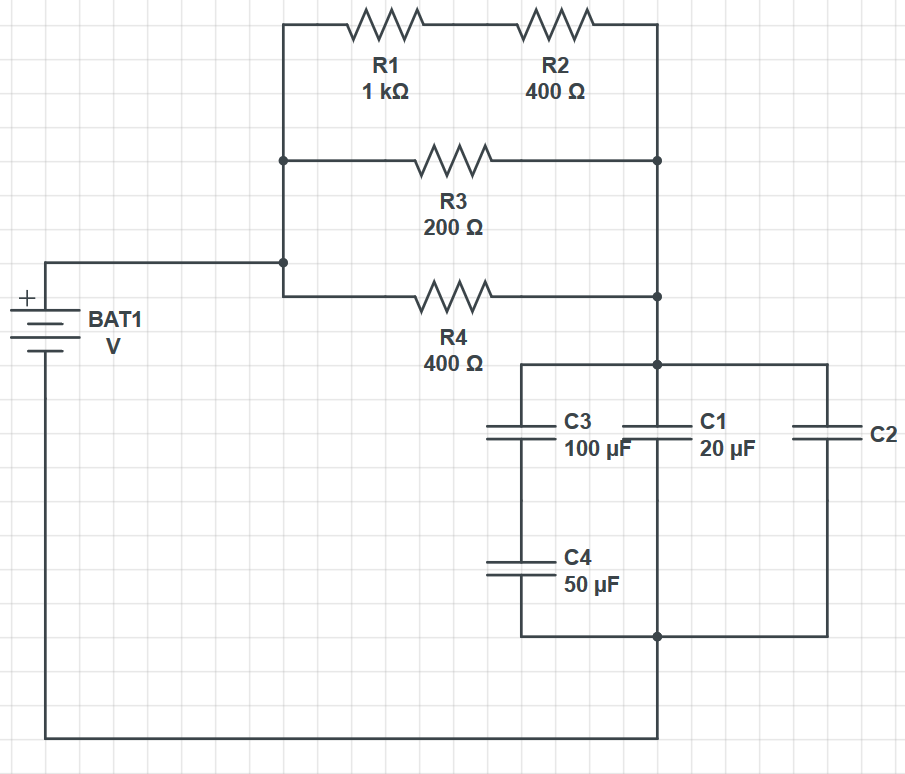
\includegraphics[width=0.6\linewidth]{lab2-session1-Cpractice}
\caption{Time constant practice.}
\label{Fig:lab2-session1-tau-practice}
\end{figure}

\begin{tcolorbox}[title=Answer]
For the first part, $C2 \approx 50\mu$F. For the second part, $C2 \approx 61\mu$F.
\end{tcolorbox}

\item If you want to keep a trace of a graph produced by the PASCO, click on the Final results tab and select which graph you want by choosing the right run in the scrolling menu of the colored triangle. Click on the camera icon on the top panel. This will take a picture that will be accessible in the journal, on the right hand side, where it can be saved as jpeg or html. Alternatively, you can also save your whole set of measurements by going to the top left tab ``File", and select ``Save As".
\end{enumerate}

Once you have completed the above manipulations, make sure to note important technicalities of the time constant measuring methodology in order to accelerate your data acquisition process for the next session. You should perform any further tests that you believe would help you better understand the RC circuit in preparation for the next session.

\begin{tcolorbox}
You may want to pull their attention towards quantifying their errors, in preparation to the next session. Note that the standard deviation from the PASCO fit is significantly smaller than that obtained from measuring the time difference at $V=V_0 (1-e^{-1})$. Discuss the disparity between the error of each methods.
\end{tcolorbox}

Resistors and capacitors can be found in the lab. Instructions about reading the resistance color-code for resistors can be found in the Appendix. We recommend that you try and read the resistance of a few resistors and confirm by using the in-lab multimeters. An exemplary circuit board that you must use during the next session will be available for you to contemplate. We recommend that you observe the set up of the circuit board and think about how you would connect the resistors and capacitors to obtain different equivalent resistance and capacitance setup.

\section{Session b}
\begin{tcolorbox}[title=Session \#2]
In this session you will help students connect their circuits and guide them through the analysis of their data.
\end{tcolorbox}
\begin{tcolorbox}
By using small time constants, we expect each measurement to fluctuate by $\pm 5$\% from the theoretical value. It may be that some  measurements don't fall within a standard deviations of the line of best fit, but the percentage error should remain small.
\end{tcolorbox}
\begin{tcolorbox}
We expect students to consider the possibility of internal impedance from the PASCO unit. We expect them to propose possible methods to extract the internal impedance of the PASCO. Testing showed that a rigorous experiment to extract the internal impedance would be too time consuming for these lab sessions.
\end{tcolorbox}
\begin{tcolorbox}
Through testing, we found that the internal impedance of the PASCO is not large enough to allow measurements of time constants of the order of 10s. To remedy the situation, one can add a large impedance to the probes of the PASCO. For more advanced students, push them to think of how the PASCO and multimeters measure voltages and hence the limitations of the setup.
\end{tcolorbox}

In this session, you are asked to build an RC circuit with a specific time constant. Your circuit will have two sub-circuits: one that consists only of resistors and another one that consists only of capacitors. You are to placed both of these in series with the PASCO source as shown in Fig.~\ref{Fig:lab2-session2-circuit}.

\begin{figure}[h]
\centering
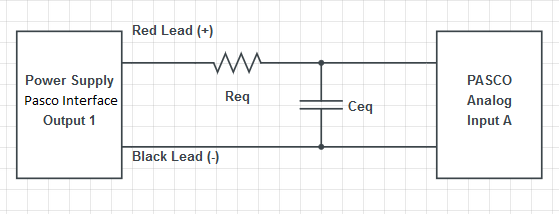
\includegraphics[width=0.9\linewidth]{lab2-session2-circuit}
\caption{RC Circuit. You are to assemble sub-circuits that produces an equivalent resistance $R_{eq}$ and capacitance $C_{eq}$.}
\label{Fig:lab2-session2-circuit}
\end{figure}

In this lab, you will only use the ``Positive Square Wave" input. Adjust them accordingly to your estimated calculated theoretical time constant for each measurement. Sometimes, the data fitting tool cannot give standard deviations: this is because the data acquisition frequency isn't properly set. Change it until you see a standard deviation in the $B$ parameter from the Curve fitting window.

There will be a few communal multimeters that allows to measure capacitance, while every team will have their own multimeter that can only measure resistance. There will be boxes containing different resistors and capacitors. Their values will be labelled but you can double-check their values using the multimeters. Note that we are using polarized capacitors and therefore you must be careful when connecting them to the circuit: the voltage input must be attached to a specific leg of the capacitor.

While every team will have to build a different RC circuit, the time constants that we are asking are of the order of ms, and therefore you will have to use the "Positive Square Wave" input from the signal generator. You have the liberty to choose different values of frequency depending on your estimate time constant. Changing the frequency of the input source does not change the time constant: this only changes the duration that the source is "turned on".

\anhkhoi{Should we tell them the two methods to confirm their measurements? Or should the TAs talk them through it to find the second way?}

To confirm your time constant measurement, you should take two approaches. The first is to simply perform charging and discharging measurements multiple times and average the given time constant measurements.

The second is to confirm your equivalent resistance and capacitance by varying time constant. Since the time constant is $\tau = RC$, if one varies the value of one of the parameters $R$ or $C$ and plot $\tau$ as a function of the varying parameter, one expects the data to show a linear trend where the slope is the value of the other parameter. By performing this test, you will firstly verify eq.\eqref{Eq:time-constant}. Furthermore, this is a complementary method to measure your effective resistance and capacitance which should match your measurements obtained by using the multimeter.

To accelerate this measurement method, each team will have 5 capacitors of $10\pm 1\mu$F and 5 resistors of $50\pm 1 \ \Omega$. Since there is a limited quantity of multimeters that can measure capacitance, you can assume that these standard deviations are correct. A summary of the equipment for this session is shown in Table~\ref{Tab:Lab2-material}.
\begin{table}[h]
\centering
\begin{tabular}{||c | c ||}
\hline
Individual station & Collective station\\ \hline
Laptop & Assorted resistors \\
PASCO 850 interface & Assorted capacitors \\
Resistance multimeter & Capacitance multimeter \\
Resistance and capacitance sub-circuit setups & \\
Five $10\pm 1 \mu$F capacitors & \\
Five $50 \pm 1 \ \Omega$ resistors &  \\
\hline
\end{tabular}
\caption{Available material for Lab \# 2}
\label{Tab:Lab2-material}
\end{table}

Document your results and argue whether or not your RC circuit has the demanded time constant. If you believe that it does, argue using standard data analysis methods. What is the most appropriate measure to characterize the error of your measurements (see ``Measurement analysis" section of the ``Basic statistics" section)? If your data doesn't produce the correct time constant, explain why. Explain what you must change in your circuit to remedy the situation. Also discuss whether you believe this experiment is adequate to obtain RC time constants. If possible, propose a better way to obtain time constants and/or decrease the error in your experiment.

\chapter{Magnetic Field of Solenoids and Coils}
\section{Learning objectives}
\begin{itemize}
\item Learn about solenoids.
\item Learn how to use the right hand rule.
\item Learn about vector fields.
\item Learn about limits.
\item Learn about electric motors.
\end{itemize}

\section{Introduction}
The goal of this lab will be to learn about real-world applications of magnetism. In particular, we will study the solenoid in the first session, and the electric motor in the second. You will use your data analysis skills previously acquired from the other labs to characterize the magnetic field of these setups.

In the first session, you will be asked to draw the magnetic field lines of the solenoid and to explain your findings in terms of the right hand rule. You will then quantitatively characterize your solenoid: you must verify the dependence of the magnetic field $B$ on the current $I$ through the solenoid and the the position $z$ from the end of the solenoid on its central axis.

In the second session, having learned how magnetic field strength varies with distance, you will now use a permanent magnet to characterize an electric motor.

\subsection{Pre-lab activity}
\begin{enumerate}
\item Question about magnetic field of straight wire
\item Magnetic field due to stacking multiple wires together
\item Force on magnetic field due to B field
\end{enumerate}

\section{Session a}
\subsection{Solenoid setup}
In this session, you will use the IOLab that you previously used in PHYS 101 last semester to measure magnetic field strengths.

Includes equipment and how to set-up the apparatus...

\subsection{Magnetic Field Lines}
Once the solenoid has been properly connected, you are first asked to draw field lines on the graph paper. For this, we will use the compass and IOLab as shown in Fig.~\ref{YY}.

First, chose at least a dozen points on the graph paper. For each point, you are to measure the orientation of the magnetic field with the compass, draw a vector line associated with your observation, and write next to the vector the measured strength of the the magnetic field. Recall that the total length of the magnetic field amplitude will be given by Pythagoras theorem:
\begin{equation}
| \mathbf{B} | = \sqrt{B_x^2 +B_y^2}.
\end{equation}
Both vector components can be obtained from the IOLab. Normally, one would draw the length of the vector in a way that is representative of the magnitude of the vector, however for the amount of vector lines you are asked to draw, we will simply write the magnitude next to the vector for this lab.

Once you have enough points, and have explored the possible orientations of the magnetic field vector lines, answer the following questions in your log book:
\begin{enumerate}
\item Draw a diagram of the solenoid with the appropriate field lines.
\item What is the magnetic field inside the solenoid? Support your claim of the field lines inside the solenoid in terms of the right hand rule.
\item What happens if you swap the connections of the solenoid? What would change? Explain this in terms of the right hand rule.
\item Do these field lines look like any known magnetic objects? Explain why this observation is true.
\item What parameters do you expect to affect the strength of the magnetic field of the solenoid? Give a brief explanation for each parameter.
\end{enumerate}

\subsection{Current dependence}
Now that you have a rough idea how a solenoid generates a magnetic field, we will quantitatively verify some of its possible parameters.

We will first verify its dependence on the current through the wires. Place the IOLab on the ramp at a fixed distance away from one end of the solenoid (not too far) as shown in Fig.~\ref{YY}. Since the power supplies yields values of current between 0 and 6A, make incremental measurements of $B$ as a function of $I$ by increasing the current by $0.5$A incrementally. Verify how $B$ depends on $I$ using your data analysis skills from previous labs. Carefully support your claim of its parametric dependence by generating a graph with some fit. 

\subsection{Distance dependence}
We will now verify the magnetic field generated by a solenoid at a distance $z$ (on the central axis) away from the front of the solenoid. The TAs will write the equation of the magnetic field of a solenoid on the board and you are asked to verify the \textbf{far $z$ behaviour} of the magnetic field of the solenoid, that is for $z>4R$ \anhkhoi{verify range}.

Place the ramp in front of the solenoid such that the IOLab sensor is centred in front the solenoid. Move the IOLab incrementally, and at each position, use the interface in order to obtain the average and standard deviation of the position and magnetic field of the measurement. You will not need to go further than 30 cm. We recommend that you perform multiple trials to obtain multiple data points.

Does your data match the equation on the board? What about the far $z$ behaviour? Discuss your results.

\section{Session b}
\Large{\textbf{WARNING!}} \normalsize The permanent magnets used in this experiment are quite strong. Avoid bringing any magnetizable (made of iron/steel/Ni/Co, ID /credit cards) objects near the magnets. \textbf{Students with pacemakers could be excused from this lab.} \\

In this session, we will study the electric motor. The electric motor is a device that converts electrical energy into mechanical energy. Electric motors and their counter-parts, electric generators, have been around for decades now and have become so ubiquitous in our daily lives that life without them would seem almost impossible. Over the years, these motors have grown in complexity and sophistication in order to perform a number of different tasks but the basic physical principles behind their operation have not changed.

The goal of this lab is to provide a general understanding of how a simple DC motor works with the hope that it might lead to a better appreciation for the more sophisticated devices found all around us. This lab is not ``complicated" to do, but will require a number of different concepts in electricity, magnetism and circuit theory to complete.

The main observable of this lab is the frequency of rotation $f$ of the motor. Similar to the first capacitance lab, you are also asked to find possible parameters that could affect the frequency of rotation of the motor.

\subsection{Electric motor setup}
Includes equipment and how to set-up the apparatus (oscilloscope)...

For this lab, you are given a power supply, an oscilloscope, an electric motor and a magnet. 
Fig.~\ref{YY} shows the schematic diagram of the setup we will use in this experiment and Fig.~\ref{YY} shows a photograph of the actual setup. To set up the apparatus:
\begin{itemize}
\item Make sure the power supply is turned off
\item Connect the leads from the coil to the power supply.
\item Instructions about oscilloscope...
\end{itemize}
\anhkhoi{Include figures}

The coil current and the voltage will be read from the power supply meters. The coil's period of rotation will be measured by a photodiode detector connected to a CRO. The photodiode emits light and detects its reflection from the shiny strip covering one side of the coil. The other side is covered by a non-reflective strip. When the coil is rotating, a signal/pulse will be seen on the CRO screen every time the reflected light strikes the detector. The period will be the time interval between two reflected signals/pulses. From the period you can calculate the frequency. The performance of the motor and preciseness of measurements are extremely sensitive to the positions of the photodiode and brushes. \textbf{Please be careful with the apparatus, and do not make any adjustments from how it was set up.}

In addition to the electric motor, you are given a magnet on a track. In the previous lab, you showed found that on its axis, the magnetic field generated by a solenoid decreases by a function similar to Fig.~\ref{YY}. In this figure, we are giving you the calibration of the magnetic field of the magnet as a function of position. You can use this to determine the strength of the magnetic field on the coil at a given distance. \anhkhoi{include calibration figure}.\\

\large \textbf{Please respect the following instructions in order to avoid damaging the apparatus:} \normalsize
\begin{itemize}
\item Do not exceed a voltage of 10 V.
\item Do not let the magnet be any closer than 1 cm to the coils.
\item It may happen that for a large enough voltage and close enough distance, the magnet might vibrate or be pulled towards the coils. Do not let it be any closer than 1 cm to the coils! Hold your magnet in place if necessary.
\item If you are using high voltages (greater than 8 V), try to move quickly through the higher voltages to reduce wear on the brushes.
\item Remember to turn off the power supply after you have finished all your measurements.
\end{itemize}


\subsection{Protocol}
Similar to the first lab, you are asked to find what parameters could affect the frequency of rotation of the motor $f$.

To do this, recall that you must isolate your parameters and vary one of them at a time to acquire data that you could analyse. As a starting point, we suggest that you draw a force diagram of the coils of the motor. Recall your answers from the pre-lab activity.

To make a measurement,
\begin{enumerate}
\item Make sure you read the previous instructions (above) in order to avoid damaging the apparatus.
\item Set the magnet at a desired position (\textbf{greater than 1 cm away from the coils}).
\item Turn the power supply to a desired voltage (\textbf{do not exceed 10 V}).
\item The coil should start to rotate, though you will likely need to flick it gently with your finger to get it started.
\item Measure the period $T$ from the time interval between two successive pulses from the CRO.
\item For better precision, you may count the time interval between a few pulses and divide it by the number of intervals to get a better value for $T$. The frequency will be given by $f = 1/T$. Note the value of f in an Excel sheet with any other relevant parameters for this measurement.
\end{enumerate}

Through discussions with your lab partners, other teams and the TA, you must perform measurements to establish a (mathematical) relation between possible parameters that could affect the frequency of rotation of the electric motor. Support your claims based on data and figures as usual.

\phantomsection
\addcontentsline{toc}{part}{Appendix}
\part*{Appendix} \label{Part:Appendix}

\phantomsection
\addcontentsline{toc}{chapter}{Introduction to Excel}
\chapter*{Introduction to Excel}

Firstly, every McGill student can obtain a free copy of Microsoft Offices software by clicking \href{http://kb.mcgill.ca/kb/article?ArticleId=5172&source=Article&c=12&cid=2}{here}. Excel spreadsheet boxes can take in strings of letters of numbers as input. If the input is a number, we can easily perform calculations.\\

\noindent \large \textbf{Spreadsheet Calculations} \normalsize
\begin{itemize}
\item To initialize the math environment, simply click on a box, and press the ``=" key on your keyboard. Press ``Enter" when you are done.
\item One can perform basic addition (+), subtraction (-), multiplication (*) and division (/) between two boxes. One can also take powers by using `` ^ " i.e. x^2 would be $x^2$. First, press ``=", click on the box of your first variable, choose one of the above manipulations and choose another box as your second variable.
\item Excel obeys order of operators: multiplication and division come before addition and subtraction. Parentheses are done first.
\item Note that the middle bar above states the equality function in terms of \textit{boxes} of the spreadsheet.
\begin{figure}[h]
\centering
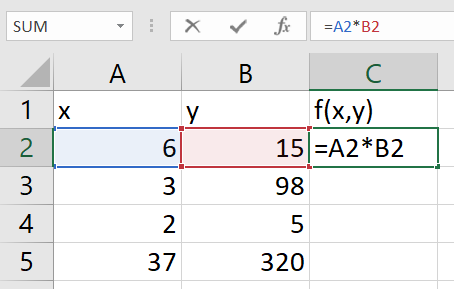
\includegraphics[width=0.4 \textwidth]{Excel-tut-boxes.png}
\caption{Example of multiplication between two variables $x$ and $y$. Notice that the selected box has a green border around which the bottom right corner has an enlarged square.}
\label{Fig:Excel-boxes}
\end{figure}
\item It is useful to separate your data into columns. In this way, say your first two columns are your $x$ and $y$ variables that were obtained from a measurement. You should compute $f(x_i, y_i)$ in another column. Doing so, after performing the mathematical manipulation that you wish, you can click the bottom right green border of a box, and \textit{pull} down to the column to apply the same function along the columns of the input variables. In the example of Fig.~\ref{Fig:Excel-boxes}, one could obtain the multiplication of each element of columns A times those of column B displayed in column C.
\item When defining a function with the intent of dragging the select-box down to apply the whole function to all elements of columns, it is sometimes useful to define a box that \underline{doesn't change} as you drag the select-box. To do so, one uses the \$ sign as in Fig.~\ref{Fig:Excel-fixed}.
\begin{figure}[h]
\centering
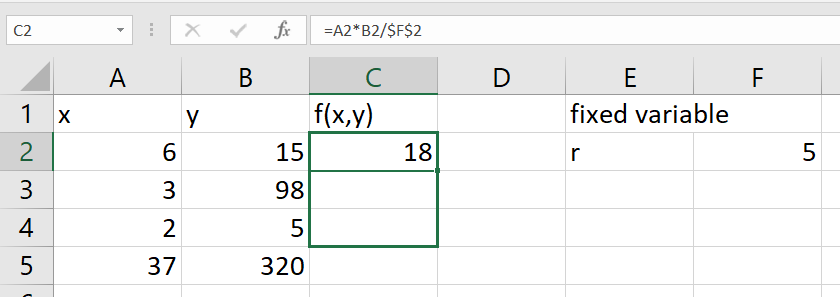
\includegraphics[width=0.8\textwidth]{Excel-tut-select-fixed}
\caption{Fixing a box value when applying a function down a column. The \$ sign before the column letter means that we are fixing the column, and the \$ sign before the row number means that we are fixing the row. One can only use one \$ sign to fix either the column or row as desired.}
\label{Fig:Excel-fixed}
\end{figure}
\item Excel also has functions that are included. Functions are called by some special command in all caps. One typically calls a function, for example the sum, as 
\begin{verbatim}
=SUM(B2:B5)
\end{verbatim}
The colon means that we take every box between B2 and B5. One could have also used that function by listing every box individually, separated by a coma. Alternatively, one could, after writing ``=SUM(", selected the boxes that one wants to be included in the function. This re-emphasizes the usefulness of arranging the data in columns.
\item Other useful functions include:
\begin{itemize}
\item \verb|=STDEV.P(x)| to calculate the standard deviation of a fluctuation population as shown in eq.~\eqref{Eq:STDev.P}.
\item \verb|=SQRT(x)| to calculate square root of $x$.
\item \verb|=Exp(x)| to calculate exponentials $e^x$.
\item \verb|PI()| to use the constant $\pi$. Note that there is no input.
\item \verb|=Sin(x)| and \verb|=Cos(x)| to calculate values in radians. The input $x$ must be in radians.
\item \verb|=AVERAGE(A2:A10)| computes the average of the boxes between A2 and A10.
\end{itemize}
There exists many other functions that could be useful.
\end{itemize}

\noindent \large \textbf{Figures} \normalsize

One can also create figures from data sets in Excel. To do so, select too columns and go into the \textbf{Insert} tab as shown in Fig.~\ref{Fig:Excel-fig-insert} to choose the type of figure that you with to display. You can choose not-adjacent columns by selecting one column, press and hold Ctrl while selecting the other column.
\begin{figure}[h]
\centering
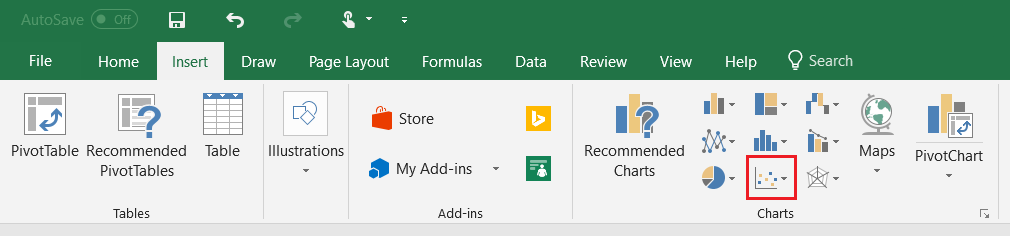
\includegraphics[width=0.8 \textwidth]{Excel-fig-insert}
\caption{Creating a plot based on some data. After selecting your data, go into the \textbf{Insert} tab and choose the type of figure that you want. The red boxed symbol is the one for scatter plots, which will most likely be your most used data display option.}
\label{Fig:Excel-fig-insert}
\end{figure}

Doing, so you should obtain something similar to Fig~\ref{Fig:Excel-fig}.
\begin{figure}[h]
\centering
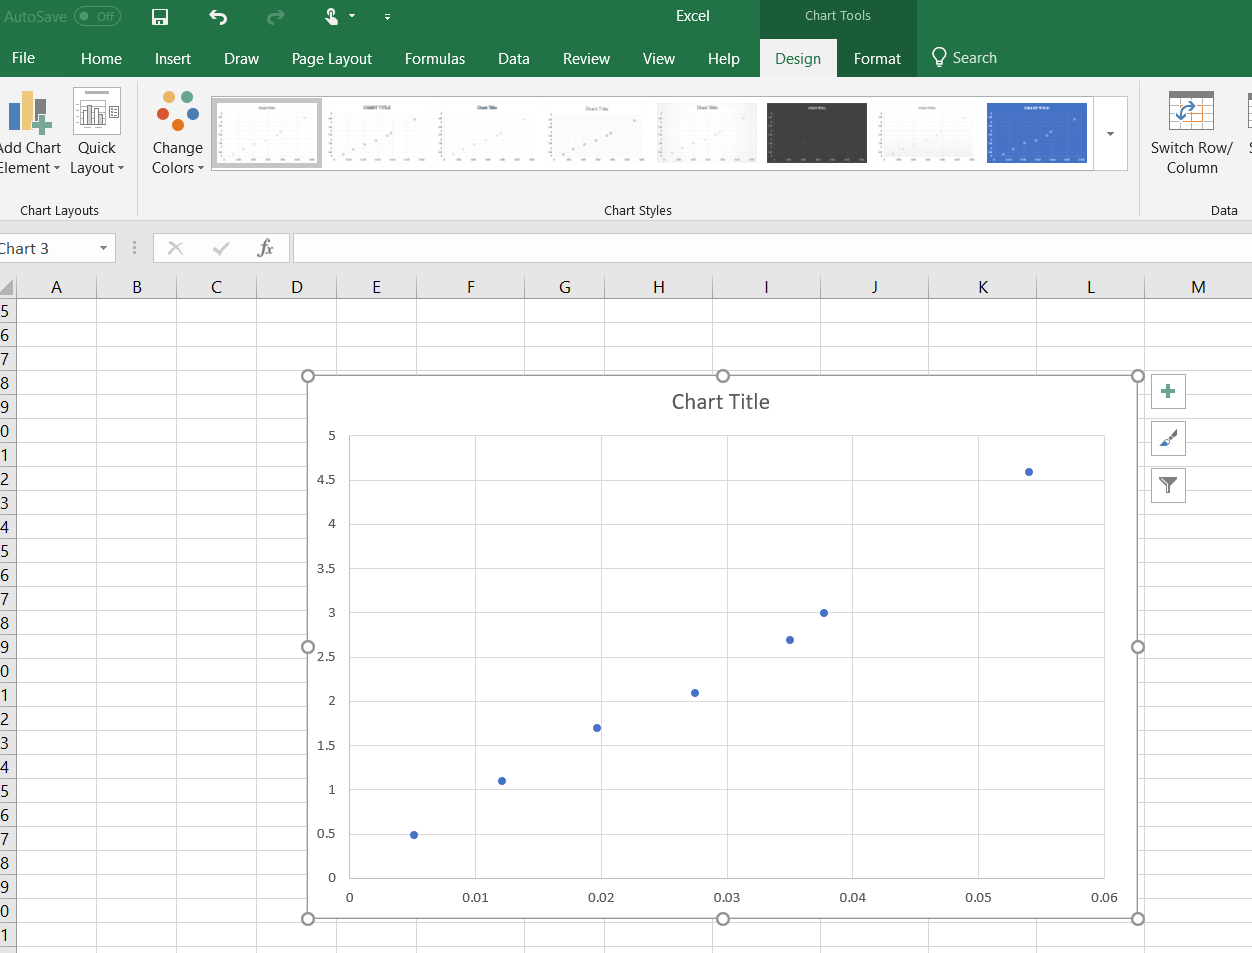
\includegraphics[width=0.8\textwidth]{Excel-fig}
\caption{Scatter plot from data}
\label{Fig:Excel-fig}
\end{figure}
From here, one can do multiple things. 
\begin{itemize}
\item By clicking the green `` + " symbol to the top right of the figure, you can add titles to your axes, error bars, a legend and a trendline.
\item By right-clicking the data points, you should see an option to ``Format Data Series". Clicking that, you will see a right bar appear, and in the ``Pain bucket" symbol, you can change the size, shape and colors of your markers.
\item By right-clicking a data point, you can add a \textbf{trendline}, in which case a right bar will also appear. Here you can choose the type of equation that you wish to fit, and if you scroll down completely, you will have the option to set an intercept, display the equation on the chart, and display the R-squared value on the chart. You can also add multiple trendlines to a single dataset to compare different fits.
\item If you right-click an empty space on the grid of the chart, you can add multiple data sets to a single chart by click ``Select Data". A pop-up window will appear with the option of renaming how your datasets will appear on the legend, and the ability to add/remove more datasets.
\item Playing around with these options, you will have the ability to change the font size of titles, colors of data points and texts, as well as change the thickness of the data points and trendlines. You can move equations, legends or other things around your chart. Don't forget that data presented must be clear.
\end{itemize}

Finally, you can add data from .txt files. To do so, go into the data tab, and in the ``Get \& Transform Data" section, there will be an option to add .txt and other types of files. Once the popup screen to import data appears, you can click on ``Edit" in the bottom right corner to have more options to manipulate your data. A useful modification is to flip your rows and columns. To do so, after clicking ``Edit", go into the ``Transform" tab in the new window, and select ``Transpose". Go back to the ``Home" tab once you are done editing your file.


\phantomsection
\addcontentsline{toc}{chapter}{Lab Equipment}
\chapter*{Lab Equipment}

\phantomsection
\addcontentsline{toc}{section}{Multimeter}
\section*{Multimeter}
A multimeter allows one to measure various electronic properties. We will be mainly interested in measuring the resistance or resistors, the capacitance of capacitors and the voltage and current of a circuit. To use the multimeter, one must attach two wires into the input and output. One can have alligator clips to attach to conducting wires more easily if necessary.

\anhkhoi{insert pic of multimeter. Box certain useful settings}

To measure the resistance, simply take a resistor, turn the knob of the multimeter to the resistance seting ($\Omega$) and attach each wire to the two sides of a resistor. To measure the capacitance of a capacitor, simply do the same as for the resistor, but turning the knob to the capacitance setting.

To measure the voltage and current of a circuit,

\phantomsection
\addcontentsline{toc}{section}{Arduino (Capacitance)}
\section*{Arduino (Capacitance)}
The Arduino unit requires the Arduino IDE software to run the desired scripts. Information about the Arduino code for the capacitance lab can be found \href{https://www.arduino.cc/en/Tutorial/CapacitanceMeter}{here}.

The setup is schematically shown in Fig.~\ref{Fig:ArduinoSchem} where the example shows two resistors: one with a resistance of $400 \Omega$, the other is unspecified. We recommend using at least $10^6 \Omega$ for the unspecified resistor: you can choose different values to vary the time constant of the RC circuit. This will change the precision of your setup.

\begin{figure}[H]
\centering
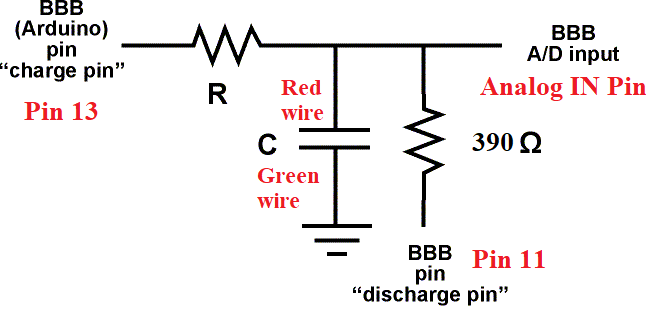
\includegraphics[scale=0.85]{CapacitanceMeterSchem.png}
\caption{Arduino circuit scheme. The labels are associated with the pins and wire colors of Fig.~\ref{Fig:Arduino-real.png}.}
\label{Fig:ArduinoSchem}
\end{figure}

\begin{figure}[h]
\centering
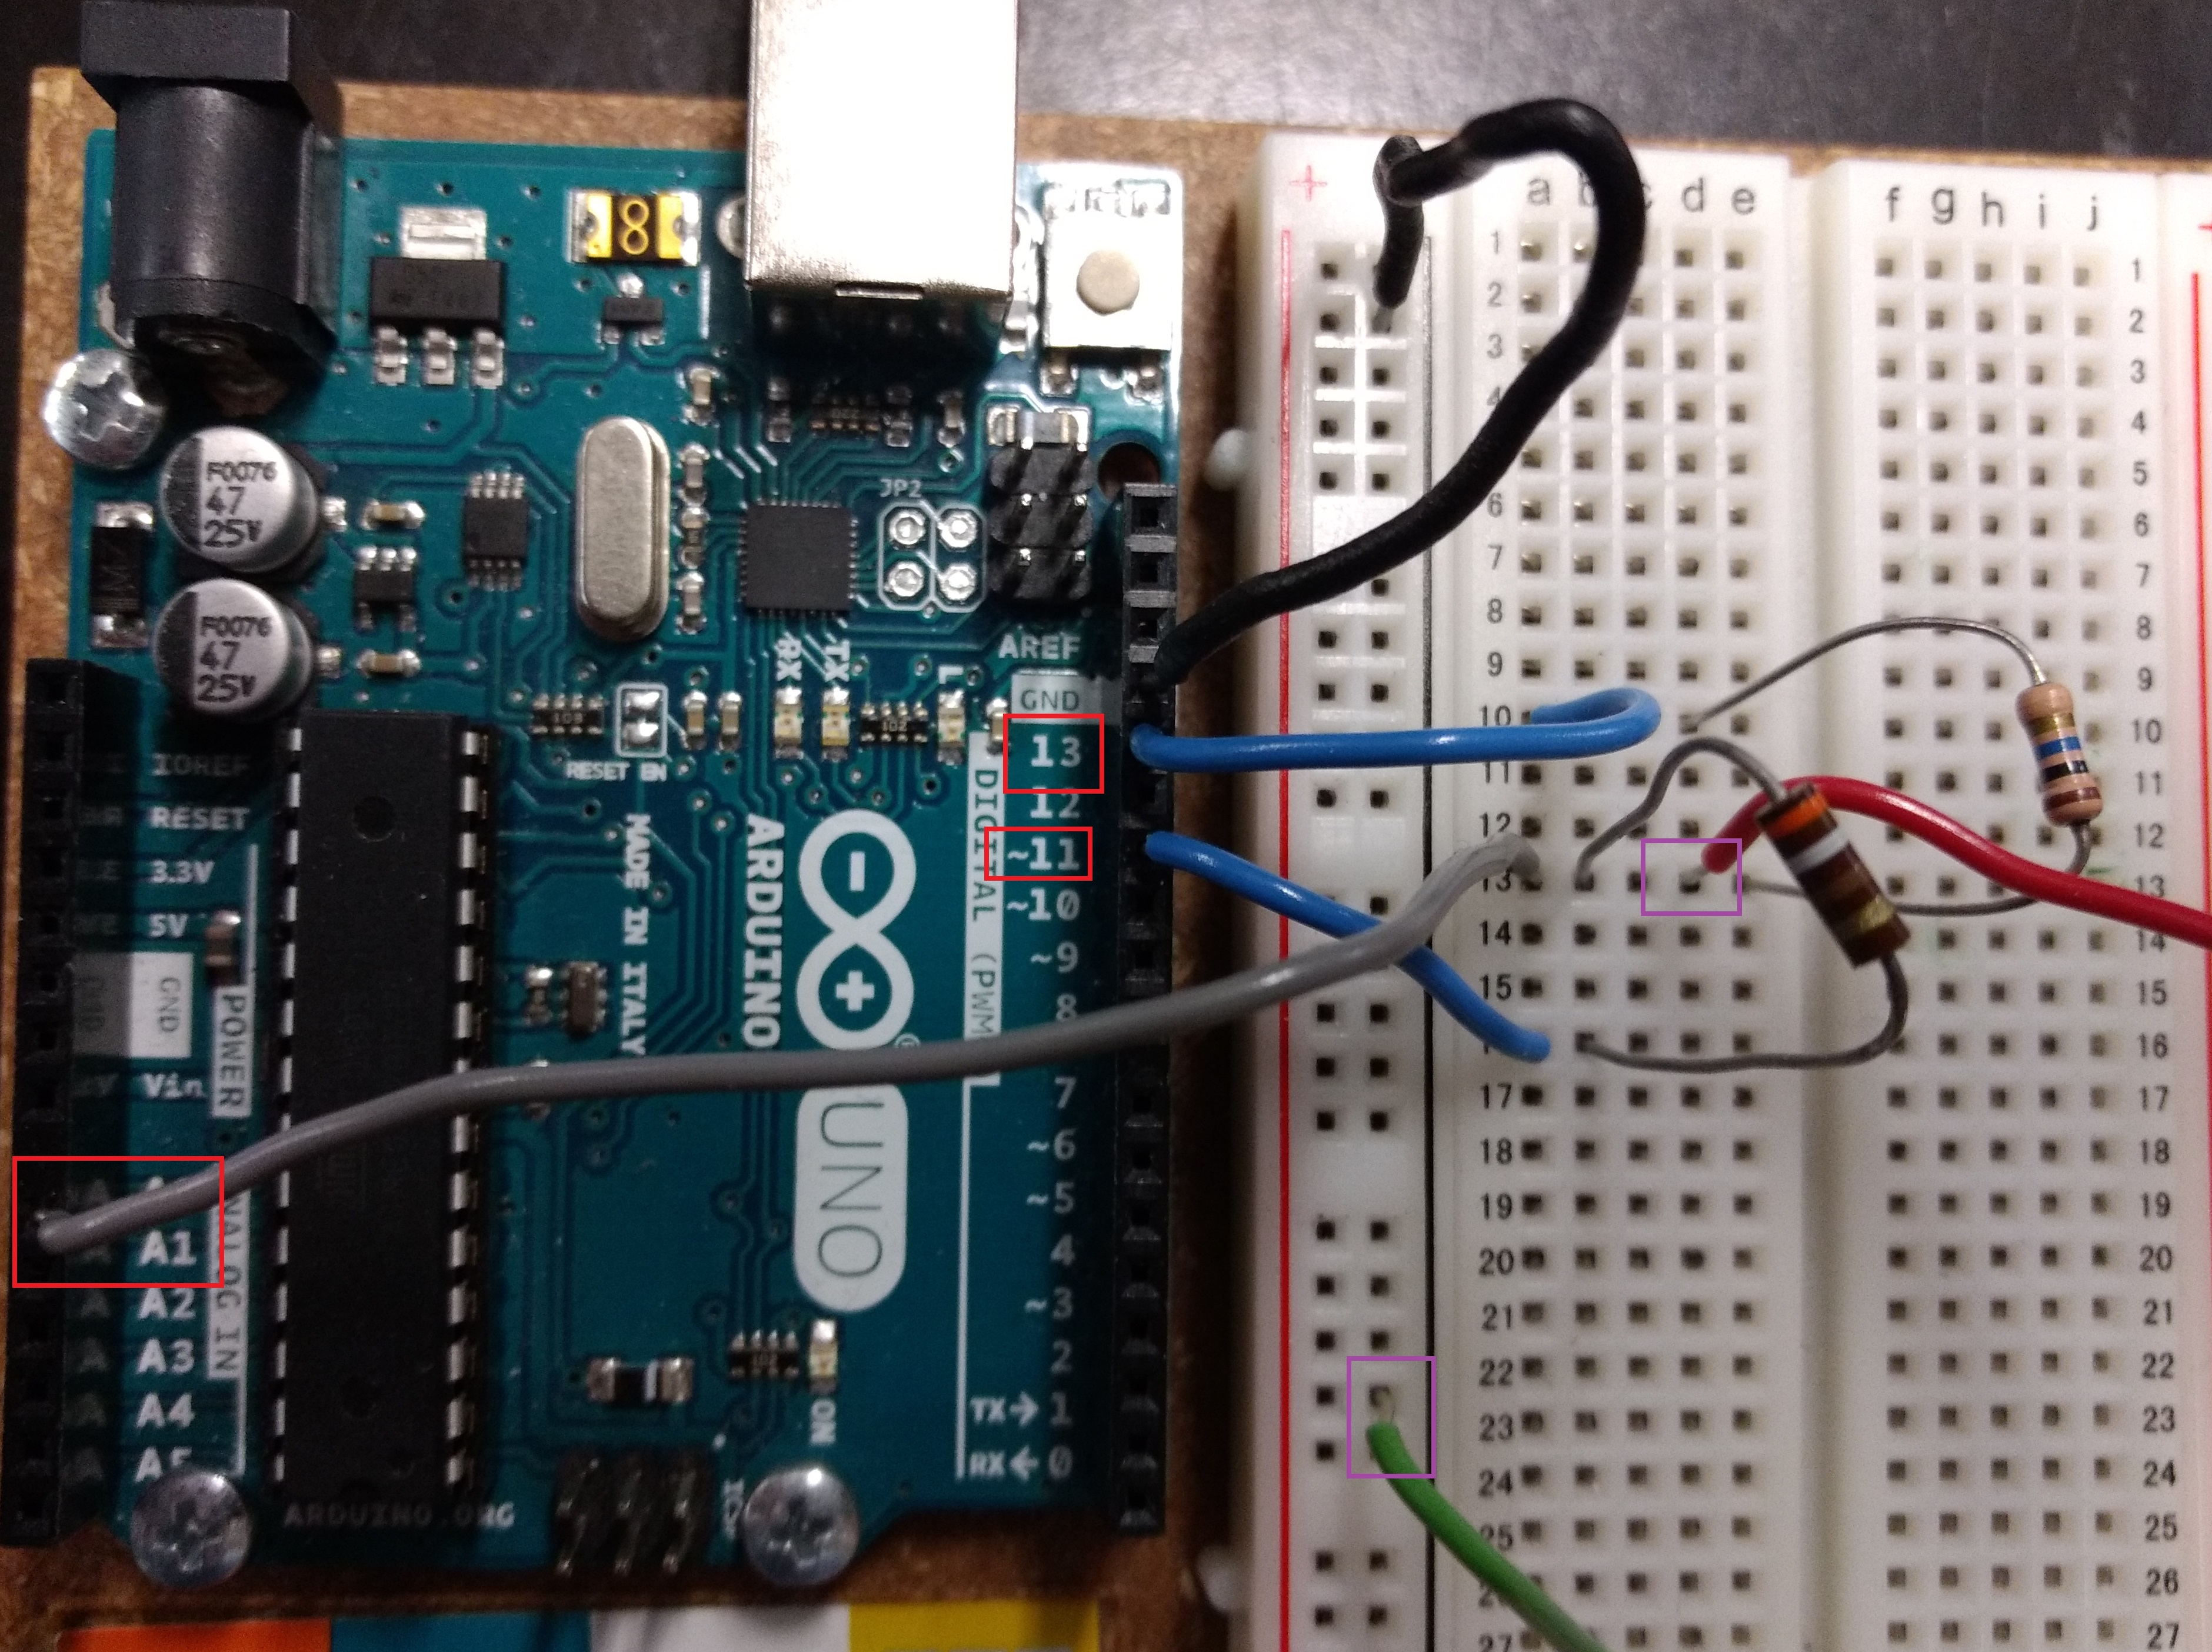
\includegraphics[width=0.8 \textwidth]{lab1-Arduino-circuit-board.jpg}
\caption{Corresponding real setup of the Arduino unit. The red boxes label the pins while the purple boxes label the wiring that should make contact to each side of the capacitor.}
\label{Fig:Arduino-real.png}
\end{figure}

To change the resistance of the resistor, you must also change the value in the Arduino script. See Fig.~\ref{Fig:ArduinoSchem}.
\begin{figure}[H]
\centering
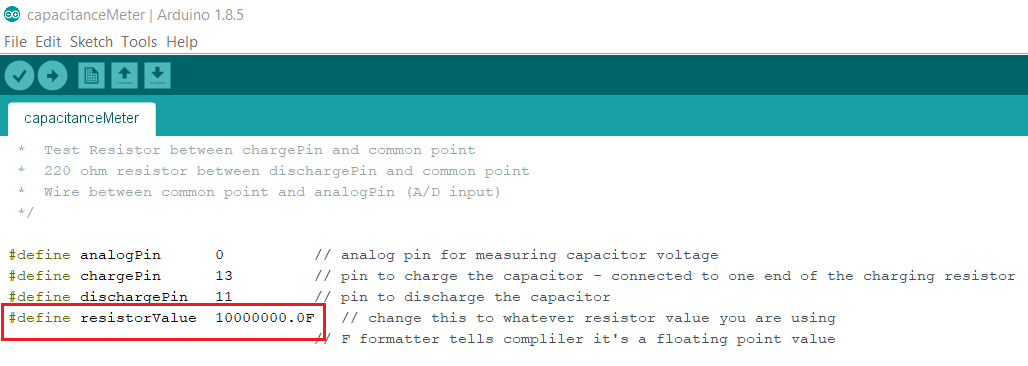
\includegraphics[width=0.9 \textwidth]{lab1-Arduino-resistance.png}
\caption{Arduino resistor value. Change the value in the red box to the resistance value of your setup. We suggest using at least $10^6 \Omega$.}
\label{Fig:ArduinoResistance}
\end{figure}

\phantomsection
\addcontentsline{toc}{section}{Reading Resistors}
\section*{Reading Resistors}

\phantomsection
\addcontentsline{toc}{section}{Circuit Boards}
\section*{Circuit Boards}
A circuit board is shown in Fig.~\anhkhoi{insert}. 

\phantomsection
\addcontentsline{toc}{section}{IOLab}
\section*{IOLab}

\phantomsection
\addcontentsline{toc}{chapter}{More statistics}
\chapter*{More statistics}

\noindent \large \textbf{Coefficient of determination} \normalsize

To determine the precision of a fit, one can look at its $R^2$ value, also known as the \textit{coefficient of determination}. Consider a dataset of $N$ datapoints with values $y_i$, $i$ going from $1$ to $N$. We define the \textit{total sum of squares} as
\begin{equation}
SS_{tot} = \displaystyle \sum_{i=1}^N (y_i - \bar{y})^2 = (y_1 - \bar{y})^2 + (y_2 - \bar{y})^2 + ... (y_N - \bar{y})^2.
\end{equation}
This is a measure of how your dataset differs from its average.

Now consider the values $f_i$ of a fit, where $i$ are the values of the fit corresponding to $x_i$ of $y_i$ value. We can also define the \textit{residual sum of squares} which is a measure of how your fit differs from your fit. This is given as
\begin{equation}
SS_{res} = \displaystyle \sum_{i=1}^{N} (y_i - f_i)^2 = (y_1 - f_1)^2 + (y_2 - f_2)^2 + ... (y_N - f_N)^2.
\end{equation}

Finally, given the results above, we can define the \textit{coefficient of determination} as
\begin{equation}
R^2 = 1 - \frac{SS_{res}}{SS_{tot}}
\end{equation}
which is a ratio of how your data fluctuations with respect to how you data differs from its fit. A good coefficient of determination is $R^2=1$. This can be computed automatically in Excel.



%\bibliographystyle{naturemag}
%\bibliography{references}

\begin{appendices}

\end{appendices}

\end{document}